\chapter{基本情况}
\section{小而精的北大工科}
2005年我们建立工学院的时候，招了一批最顶尖的学者，也对工学院有很多期许。然后我们就面对这个问题——我们北大要做什么样的工科？这个工学院是要做什么样的工科？当时工科有两种模式，一种是MIT的，它是那种大而全的工科；另一种是Caltech模式，这是钱学森的母校，它是一个体量很小的学校，但做出了相当出色的成果。

于是我们决定走Caltech的道路，做出小而精的工科，做最前沿的、对未来可能有影响的东西。当时提出的说法是“science based engineering”，这个说法至今我们还在用。我的理解是，我们说engineering，就是说我们要把一个东西造出来，但这个science，强调的就是不要按别人的路造出来，而是要创新性地、从0到1地做出新的东西。
\begin{flushright}
	——摘自工映青春公众号，唐少强老师访谈《从零开始的力学生活》

\end{flushright}

\vspace{10pt}

近几年学院在科研方向上仍然贯彻了“小而精”的理念，老师们做的方向各有千秋，作为工学院建院基础的力学是基础学科，在现在这个时代要想取得长足的发展，必然需要进行学科交叉；这也是学院目前各学科发展的大趋势。除此之外，2025年3月，学校成立北京大学工学部，由工学院（本科生学院）、力学与工程科学学院、先进制造与机器人学院、材料科学与工程学院、未来技术学院、环境科学与工程学院组成。

\section{工学院的新鲜血液}    
\subsection{招生人数与人员分布}
从北京大学的招生工作、校园开放日咨询人数中，我们可以明显感受到近年理工科名额的增加，以及工学院人数的逐年增长。这也是学院发展、招生政策、经济形势、社会环境的不断变化所共同决定的。工学院与环境科学学院2010至2026年本科生招生人数见下图。近三年工学院的数据为：2024级262人（其中强基生约180人）、2025级369人（其中强基生245人）、2026级411人（其中强基生245人）。

\begin{figure}[H]
	\centering
	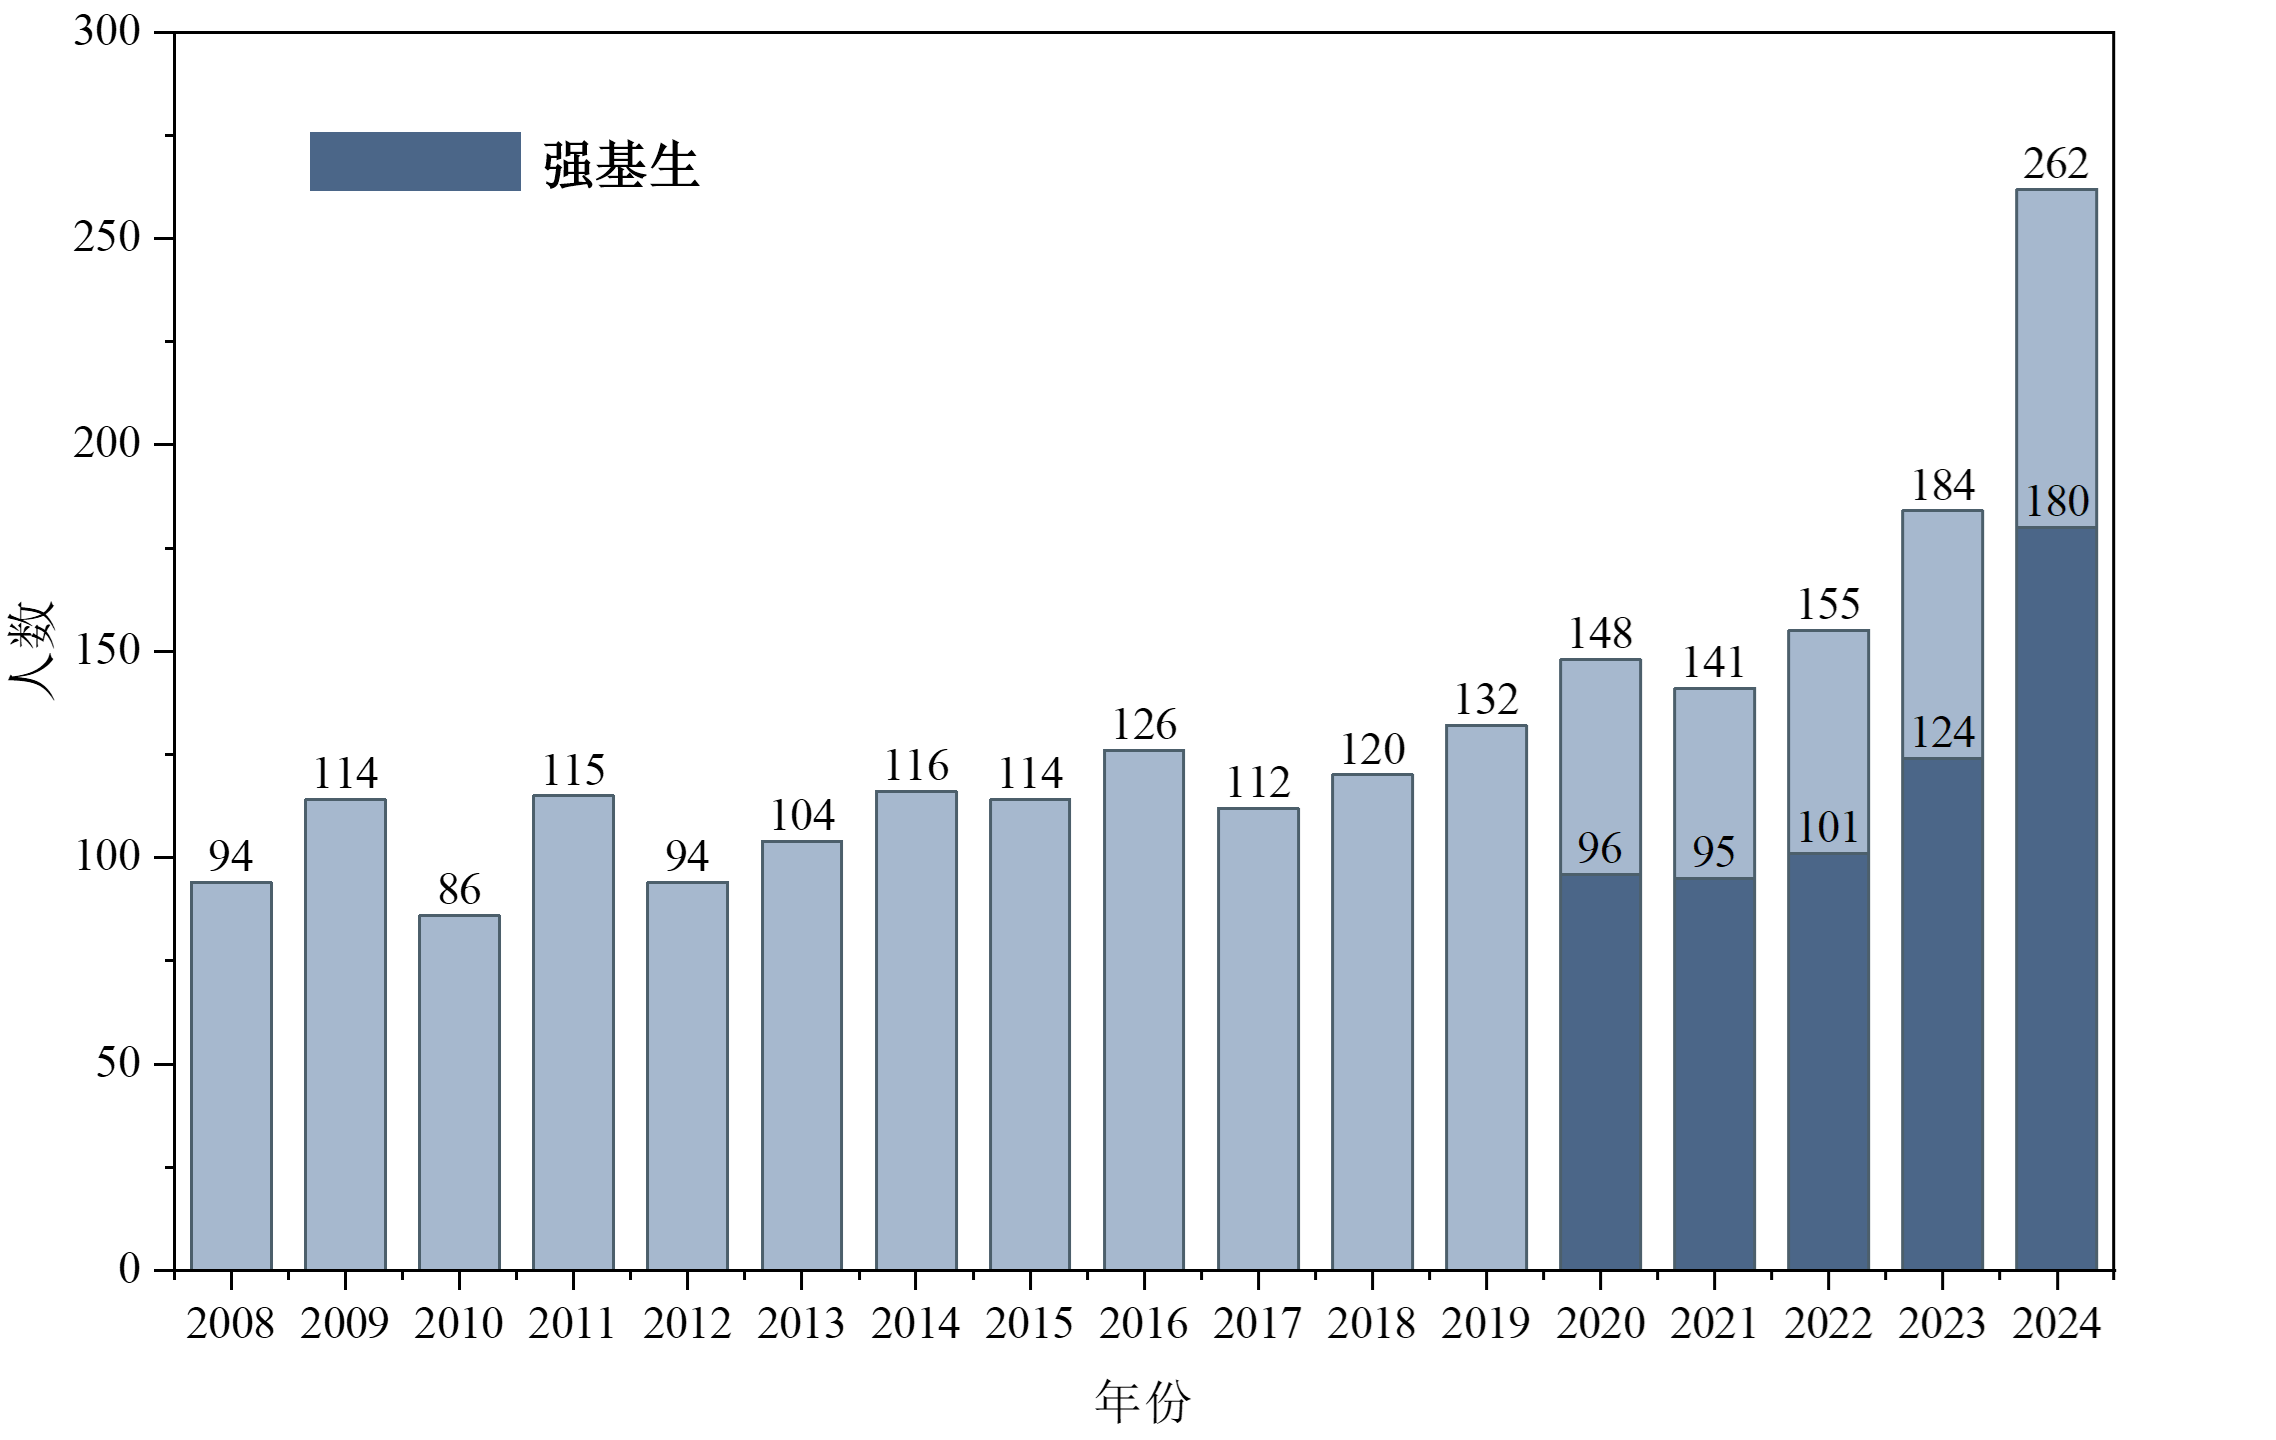
\includegraphics[width=0.7\linewidth]{assets/人数图.png} %需要重新制个图
	\renewcommand{\figurename}{图}
	\caption{工学院近年本科生招生人数}
	\label{fig:enter-label}
\end{figure}

\begin{figure}[H]
	\centering
	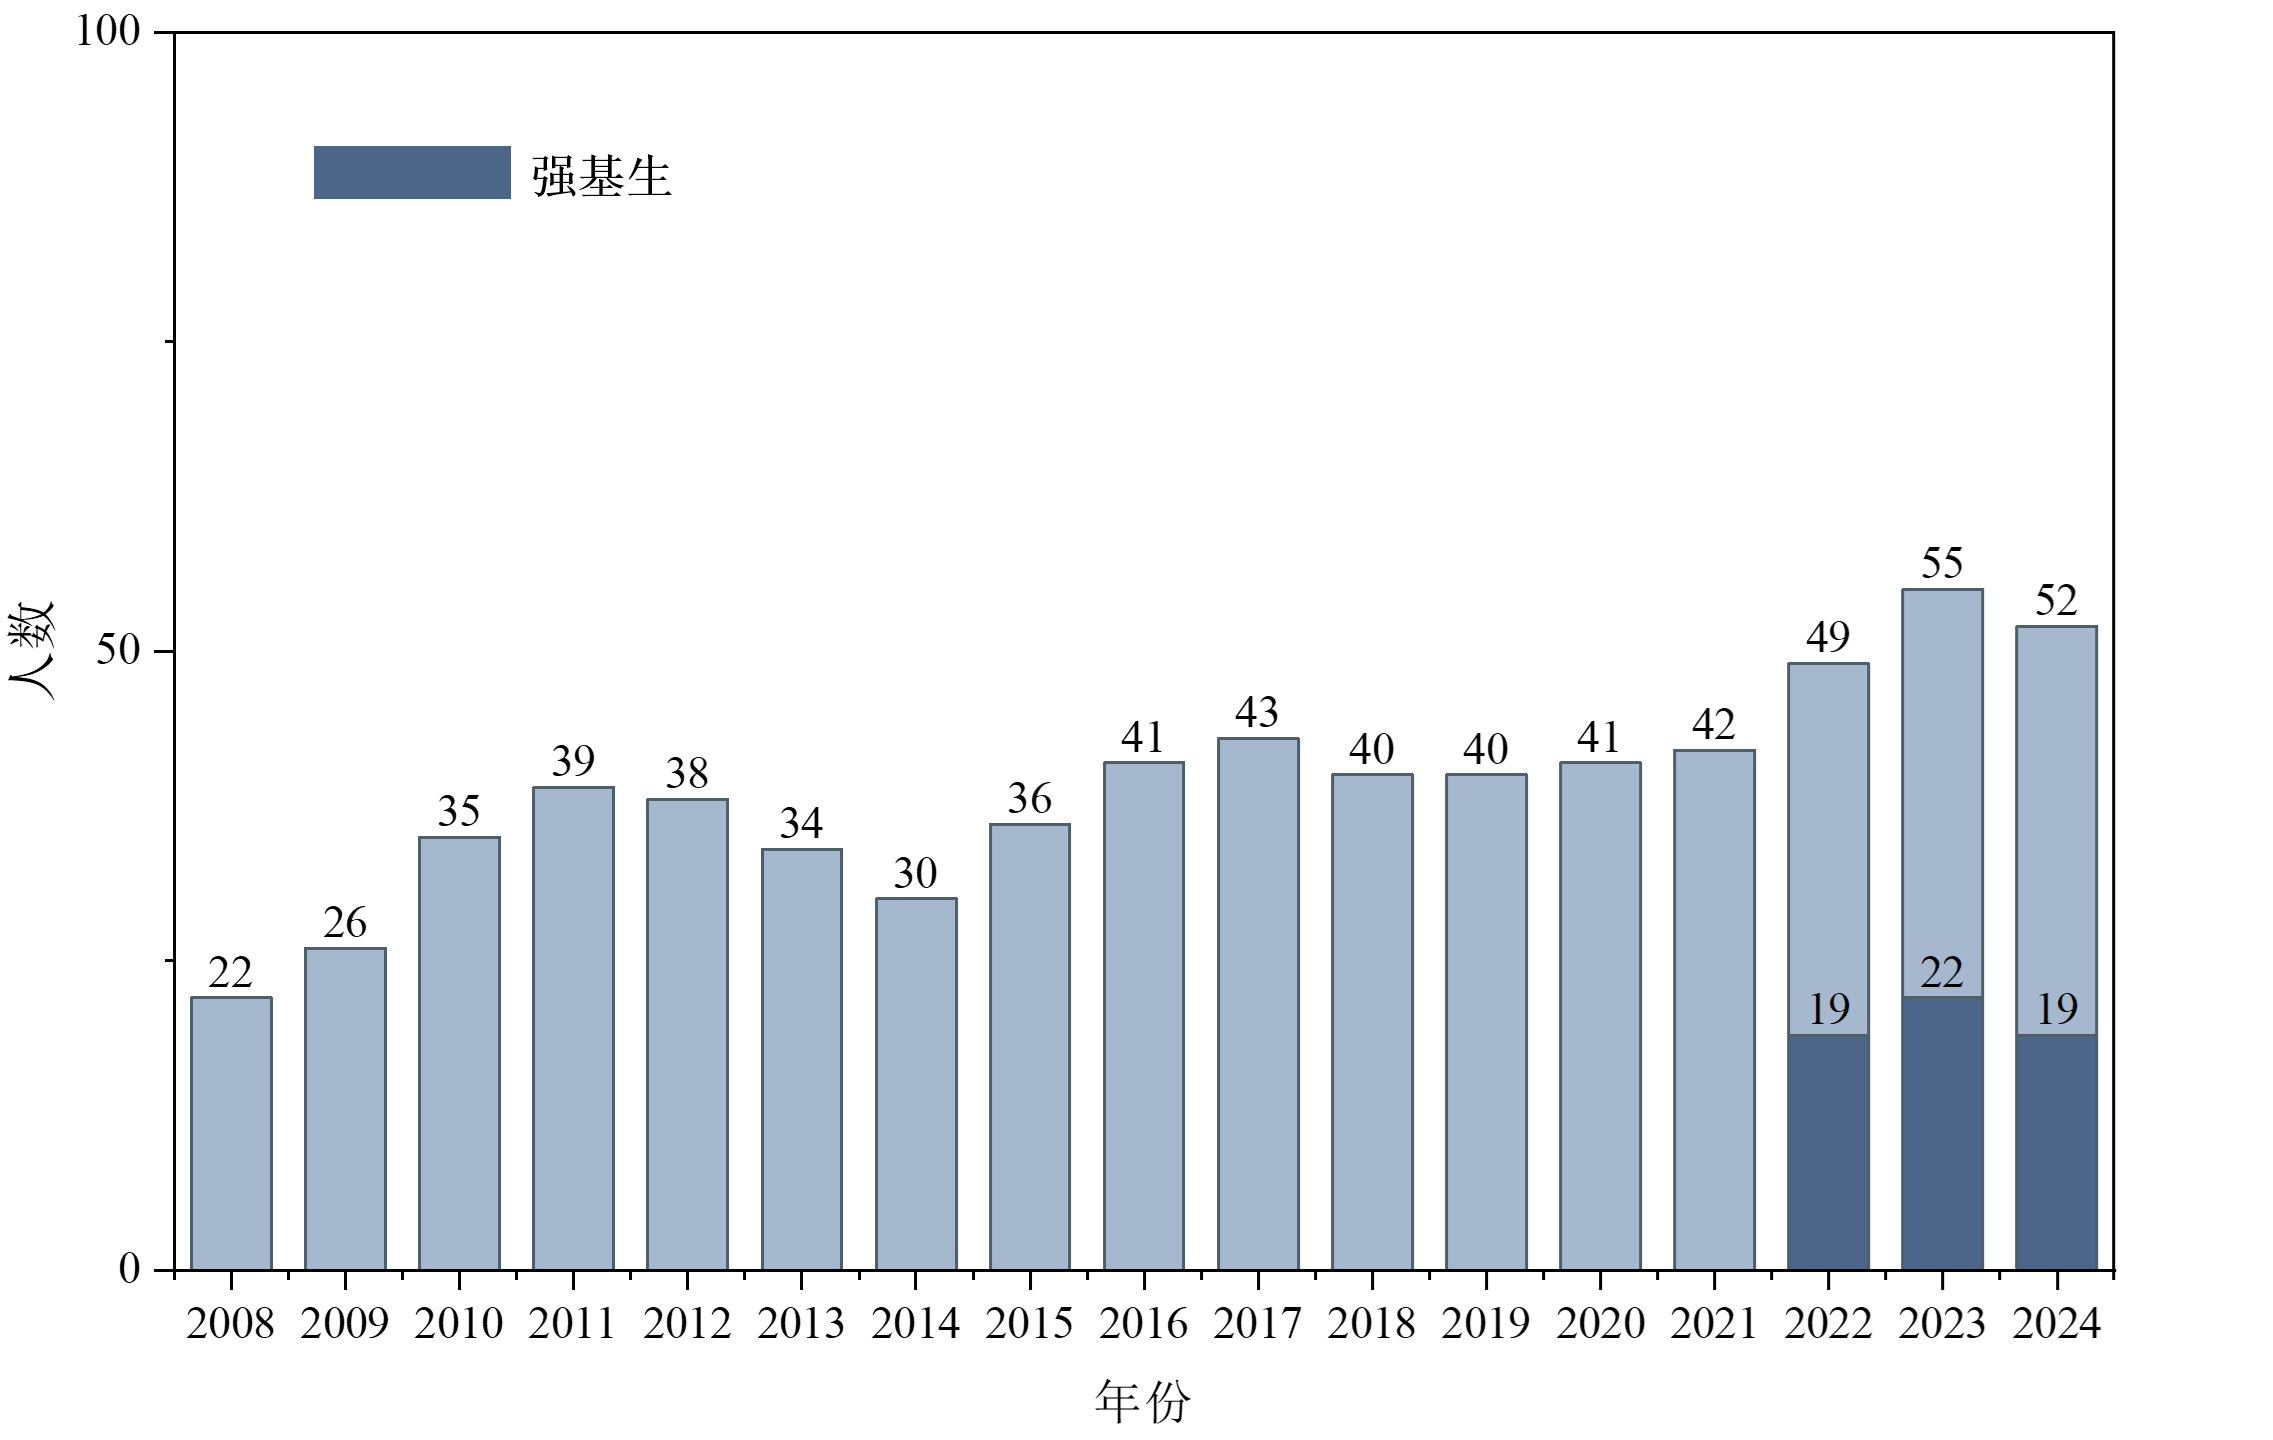
\includegraphics[width=0.7\linewidth]{assets/环科人数图.png} %需要重新制个图
	\renewcommand{\figurename}{图}
	\caption{环境科学学院近年本科生招生人数}
	\label{fig:enter-label}
\end{figure}

可以看出，由于强基专业的增加\footnote{2024年新增化学（材料科学与工程方向）、生物（生物医学工程方向）两专业}、其他院系并入\footnote{2025级环境科学与工程专业本科生的加入}和基础学科扩招，近年来工学院本科生招生人数正在稳步上升。

\vspace{10pt}

大一末分专业方向的时候，每届的同学选择也大不相同。例如：2019级，新设立机器人工程方向，50人左右选择了该方向；2022级选择理论与应用力学方向人数最多；2023级对生物医学工程方向的热情又有所提高；2024级则又对机器人工程方向兴趣较高。每学年末，工学院会召开年级大会说明各专业方向的意向人数，届时同学们可以了解到本年级选择方向的大致趋势。笔者想要指出的是：虽然工学院近年来招生人数不断上升，对同学们的学习生活产生了一定影响，但工学院方向众多，总人数的上升并不一定意味着前路“过于拥挤”，而是可能带来一些新的机遇，例如更充分的学科交流与学科融合。我们希望大家客观评估这一现象。

\subsection{工科试验班与强基计划}
工学院主要从两条轨道录取新生：工科试验班（此类同学后称“工试同学”）和强基计划（此类同学后称“强基同学”）。这两类学生面临的政策有部分差异：

\vspace{10pt}

第一，院系转换。强基计划原始文件中规定：由强基计划录取的学生原则上不能转专业。但在这一点上北大校内政策相对宽容：强基计划专业内部可以互转。工试同学原则上没有转专业限制。

\vspace{10pt}

第二，推荐免试攻读研究生。工试同学走传统的保研路径，强基同学走转段路径。强基同学自带转段名额\footnote{转段名额什么条件下被取消，请自行查找}，而GPA在推免线上的工试同学才能获得推免名额\footnote{针对2024级及之前的同学而言。2026级政策尚不明晰，但也一定和成绩相关，因此大家仍需保证较好成绩}。但无论工试同学或强基同学，推免之后找老师接收这一步，都需要自己进行。在接收方，强基同学存在限制：强基计划有委托培养性质，也就是说，北大的强基生只能保送本校攻读研究生，而工试同学可以找其他院校的老师接收自己。此外，强基计划和工科试验班的同学都不限制考研和出国。

\vspace{10pt}

第三，培养方案。详见教务部官网《北京大学本科教学计划》或工学院官网上的培养方案，其中强基与工试的培养方案会分别列出。

\vspace{10pt}

以上提到的事项（尤其是强基同学）每年具体政策都可能有变化，所以希望大家多多关注相关消息。

\section{细谈本科专业}
以下介绍工学院的七大本科专业方向和环境科学学院的五大本科专业方向，主要采用向高年级学长学姐约稿介绍的形式，内容仅供参考。尤其是与培养方案和修读课程相关的问题，稿件中学长学姐们都以2024级及之前的培养方案作为参考。因此，请同学们在仔细阅读的同时独立思考。不理解或与现行方案有出入之处，还请进一步咨询老师或学长学姐。
\subsection{理论与应用力学}
\subsubsection{（1）2021级\ 谢谊锋}
\textbf{P1 理力专业学习内容}

这里分为四个部分讲解：

\vspace{10pt}

\textbf{第一部分为政治课、英语课、体育课、通识课等课程}，这一部分课程可以有三种心态进行学习：（1）完成毕业学分。北大本科毕业要求学生必须修完这类课程，所以可以选择任务量较少的课程，满足毕业要求。（2）自己感兴趣的方向内容。北大在这些课程的开设上具有很大的广度，所以如果有正好在兴趣点上的课程，可以自由选取。（3）通过这类课程提高成绩。目前对于非强基生而言，保研的推免资格和课程成绩相关。且课程成绩越高，在学年的评奖评优中也有优势。另外，工学院较为重视专业课的学习成绩，所以对于这部分课程，同学们可适当避免那些需要投入过多精力的课，而可以选修一些给分较好的课程\footnote{当然，也会比较难抢上}。

\vspace{10pt}

上述三种心态可能同时存在于一门课程中，这当然是比较理想的情况。但是哪怕不感兴趣，不想在这类课程上花太多心思，也当然是在工院同学中普遍存在的心理，大家不必焦虑。

\vspace{10pt}

\textbf{第二部分为数学、力学、计算机的基础专业课}，下面列举了部分课程：
\begin{itemize}
	\item 数理基础课程：\\数学分析（一）（二）（三）、线性代数与几何、高等代数、常微分方程、数学物理方法（上）（下）、概率论、数理统计……
	\item 力学基础课程：\\理论力学、材料力学、弹性力学、流体力学……
	\item 计算机基础课程：\\计算概论、数据结构与算法\footnote{26级及以后本课程改为人工智能与算法设计}、计算方法……
\end{itemize}

这类课程的具体工程应用性不强，相反，其强调的是理论与概念，对于部分同学来说不是那么直观，甚至是难以理解的。但是希望同学们能够认真地学习这部分专业课，因为这部分知识，对于未来进入到需要数理知识应用的相关场景中时，会有极强的核心竞争力。同时，学院也十分重视这一部分的学习。所以，对于未来希望升学进修的同学，这一部分的学习情况是极为关键的。

\vspace{10pt}

在我的感受中，我是比周围人的理解能力要差一点的人，弄明白一些抽象概念所花的时间比优秀的同学要多一点。但是对于工学院的课程，只要肯下功夫，都是能够弄明白的，所以同学们也需要有自信心。

\vspace{10pt}

\textbf{第三部分为自主选修课}，这类课程同学们可以在全校范围内选课\footnote{注意，部分课程不计入自主选修课学分，详情参见培养方案，或向教务老师确认}。大家可以根据自己的兴趣、科研要求进行更加针对性的学习。

\vspace{10pt}

\textbf{第四部分是工学院的实验课、基础物理课程}。这类课程和工学院专业的关联性较弱，但是实际应用性很强，并且能够锻炼同学们的数理思维，也建议用心学习。

\vspace{10pt}

\textbf{P2 专业未来}

本科就业：

优势很弱，因为同学们花费了大量精力在抽象的数理知识学习上，较为缺乏具体的工程应用经验。并且本人身边的、在理力方向的同学几乎没人抽出精力去企业进行实习。另外，本科学习阶段，同学们的数理基础是比较“泛”的。例如，在固体力学这一块，同学们学到弹性力学便结束了；对于更深层次的塑性力学、断裂力学等课程的知识是没有掌握的。所以，想进入到某一方向的头部就业岗，除了教育培训，其余对口程度都很低。此外，本人也接触过某里、某方等头部企业的研发岗，我认为其工作内容对于我们学习到的这些抽象数理概念利用率低，而工作重心是在满足甲方要求的前提下，用最低的成本和最简洁明了的、最安全稳定的、最高效速成的方法完成甲方要求的项目。当然，北大文凭还是很强的敲门砖，并且同学们的学习能力也很强——这是我们的优势区间。

\vspace{10pt}

升学科研：

这是工学院大部分同学的选择，同学们通过在工学院本科阶段的学习，正如我前面提到学习的科目是很“泛”的，所以同学们是很可能找到和自己兴趣、能力相匹配的科研方向的。并且在这一阶段，可以将之前学习到的数理知识这一“内功”练就为一门独特的“外功”，将核心竞争力培养得更加具体化。

\vspace{10pt}

\textbf{P3 学习体会}

成熟的培养方案：

得益于力学系的悠久历史，本培养方案中的数理课程甚至是北大很多任教老师上过的课程，也是很多优秀毕业学长学姐们上过的。因此，经过时间长河的检验，这一培养方案在培养数理基础认知上是极为成熟的。同时，这一培养方案与具体内容也是不断革新的，保证了同学们可以在掌握基础的同时，对于力学相关前沿问题也能够有更加全面的认知和更为广阔的视野。

\vspace{10pt}

学习过程是十分辛苦的：

无论是本科生还是研究生阶段，力学系的学习都是需要同学们花费大量时间和精力的。相比其他方向的同学，力学系的卷度是更高的。力学系同学若希望取得较好成绩、专业排名，则需花费极大的精力。即使是像我这样大多数数理课程在优秀以上、自己擅长的数理课程能拿90+的同学，也是极为刻苦的。并且，以我对头部同学的观察，他们更加用功。

\vspace{10pt}

对力学数理知识有敬畏之心、好奇之心，并以在其中探索为乐，同学们的付出是可以得到回报的：

包括我在内的大部分同学，都认为我们在数理基础知识学习上投入的时间精力是得到了具有极强幸福感的回报了的。具体内容的确因人而异，所以这一部分我不具体展开描述，就留给同学们自己去发现吧。

\subsubsection{（2）2021级\ 杨铮昊}

传统的力学专业分流体和固体两派。我们最早会在大二下学期接触到的材料力学，就是固体力学的范畴，而直到大三我们才会通过两门必修课——流体力学（上）、流体力学（下）——入门流体力学这门学科。我挺建议对固体力学不是很感冒的同学，提前了解一下流体力学的内容，或许你就能更早发现自己的兴趣其实在流体。除了这两派以外，工院的力学与工程科学系还包括了许多其他的力学分支，如生物力学、力学系统与控制，也包括如流固耦合等一些交叉学科。这些方向需要学习的内容都不会出现在培养方案的推荐课程内，所以建议想要探索的同学尽早去联系对应的老师，寻求指导和帮助。

\vspace{10pt}

理力专业的课程方面恰如其名，围绕着“理论”与“应用”两个主题。在低年级优先学习的数学课和力学课都是为了打下扎实的“理论”基础，而大二下学期的材料力学实验，才正式开启“应用”的实践。如果学习理论课程时没有那么得心应手，不妨多去尝试一些实验课。这里的“实验”并不仅限于实验室里的实验，也包括那些需要动手编程的数值模拟实验。因为在未来的科研中，真实实验和数值实验都是推动科研的重要手段。

\vspace{10pt}

理力专业的课程难度总是被排在第一，因为比其他专业多出一些“更难”的数学课。但对于大多数专业而言，要想行稳致远都离不开扎实的数理基础，而理力专业只是更多强调了这一点且体现在了课程设置上。所以无论是选择哪个专业，基础数学课都一定要认真学习，力求扎实掌握。

\vspace{10pt}

有玩笑说各行各业都有理力专业的学生，这其实不假。通过本科阶段的学习，理力专业的学生应该有信心收获较为扎实的数理基础和动手能力。今后无论是在哪个领域从事科研或是就业，二者都能提供强大的竞争力。另一方面，如果你能够尽早地确定未来的奋斗方向、尽快入门并启动，更是一件好事。所以本科阶段除了沉淀和积累，很重要的一点就是多向外探索。

\vspace{10pt}

作为在此专业学习已达三年之久的“老登”，我还是感觉很幸福的，因为无论是老师还是同学都特别友善包容，让我既能在良好的学习氛围中收获满满，又敢于做出许多探索和尝试。但如果这个专业不适合你，同样放心寻求老师的帮助就好。

\subsubsection{（3）周培源班}

周培源书院（或周培源班，后简称周班）是工学院理论与应用力学专业方向专门开设的一个小班。有关招生政策基本信息，请有意向的同学多多关注学院官网报名通知，也可通过12月学院举办的工学嘉年华、大一下学期举办的若干次选专业指导讲座进行了解。

\vspace{10pt}

以下是周班的学长给大家作的补充介绍：

\textbf{周班介绍\quad 2021级 钱骏飞}

\vspace{10pt}

\textbf{\textbf{一、发起周班的动机及培养目标：}}

秉承“培本固源，笃行秀出”的理念，旨在培养出具有深厚数理基础和人文素养、追求长远科学目标、能够引领力学学科及未来新技术创新发展的杰出人才。

\vspace{10pt}

\textbf{\textbf{二、周班与普通班培养的差别：}}

目前周班同学接受的培养方案和普通班是完全一致的。在课程上的差别是，周班同学接受的是小班化教学，授课内容会略多于平行班，课程的考核难度也会较高。考虑到周班的同学们都很优秀，课程都是不限优秀率的。不过客观来说，给分并不是很香。如果大家希望的是更好地打牢自己的数理基础，多和身边优秀的老师同学们交流，同时对分数不是特别care，则非常建议大家来周班进行学习。但如果之后有出国的意愿，或者对分数看得比较重的话，一定要慎重选择，在周班想取得特别高的分数肯定是要比普通班难好多的。

\vspace{10pt}

除此之外，周班的一大优势就是灵活。每隔一段时间\footnote{大约是一学期一次左右吧}，周班的主管老师们会和同学们进行交流，询问一下同学们目前的学习情况，以及对课程进度的一些看法。如果建议得当的话，很有可能会进行一定的课程改革，比如将某些课提前一学期进行学习，或缩短/增长学时。在选课方面，周班可以进行课程替代。例如，国家精品课基础物理实验，就可以通过选修数院的实变或微分几何来替代。原则上说，必须要选取难度更高的课才能进行替代。至于具体到哪门课可以用哪门课来替代的话，最好要向周班主管老师荣起国老师询问确认好，并且经过教务老师同意。整个流程操作起来虽然略显复杂，但是真的很有用！

\vspace{10pt}

学习之余，活动也是不少滴！周班会为大家尽可能地安排讲座、报告等活动，带领同学们充分了解科技前沿进展，帮助大家认清未来可能从事的科研方向。假期会不定期组织同学们出国参观，并进行学术等各方面的交流，例如之前五一去了马德里和巴黎，暑假去德国等等。综上所述，课余生活还是很舒服的！

\vspace{10pt}

进入周班的门槛并不高。只要大家数理基础别太烂\footnote{会有个面试，别被老师拷打得太狼狈一般就没问题}，愿意接受这种培养方式，几乎就能成为周班大家庭的一员。

\vspace{10pt}

\textbf{\textbf{三、周班的转入转出机制}}

对普通班的同学，想在周班选拔之后进入周班也是可以的。你需要提前与周班的主管老师们联系好，征得同意后达到一定条件即可转入。周班的同学们倘若迫于课业压力而想转去平行班的话也是可以的，与老师们提前沟通好就行。

\vspace{10pt}

值得注意的一点是，普通班的同学可以选修周班的小班课来替代普通班的课，但周班的同学不可以修普通班的专业课来替代周班的专业课。一旦如此操作，便会被视为退出周班。

\subsection{工程与科学计算}
\subsubsection{（1）2021级\ 吴秉宪}

在我的理解中，工算方向的教学目标是培养一批兼具数学、力学基础和计算机编程能力的同学，初衷是为工业软件的设计和工程领域的计算任务积累后备力量。因此，工算的培养方案同时包括了数学分析、线性代数、高等代数、常微分方程等数学基础课，理论力学、材料力学等力学基础课，计算流体力学、计算固体力学等结合了计算背景的力学课，以及一系列与程序设计或优化方法有关的课程。

\vspace{10pt}

下面我仅站在个人立场分享我在工算方向学习三年以来的一些心得。

\vspace{10pt}

工算课程所涉及的范围较广，且很多课程之间关系不大，例如并行程序设计、计算机图形学、工程CAD、机器学习基础等。每门课基本都是一门全新的学问。这一点容易让人感到矛盾。一方面，我们能在本科阶段接触到计算机在不同子领域的应用，对完全不同的技术都有所涉猎，便于探索自己感兴趣的方向；另一方面，课程的广度不可避免地造成深度的欠缺，每门课可能只能帮助我们窥见一角，想要深入挖掘还是需要自己在课外花额外的时间。而且课程的广度意味着培养方案前后衔接得不十分紧密，每门课想学好都得花足够的时间。对于我来说，培养方案中的肯定是存在屑课的\footnote{这就需要灵活运用课程测评来避雷了，樂}。但我并不介意这样的培养模式——本科期间能够多尝试一些方向是一件好事。

\vspace{10pt}

那么，什么样的同学适合选工算？我们当时分流时，除了理力方向占绝对优势外，最受欢迎的应该就是工算了。我想，这可能是因为那时计算机热潮仍然占据主流。随着现在新能源、生医工、新材料的需求和热度升高，近两年几个小方向的人数几乎都差不多了。我认为在这样的趋势下选专业时，自己的生涯规划是最重要的。对于有明确目标或者兴趣要去某个行业的，就不必再看接下来的建议，只管在契合的领域大胆冲就是了。因为工学院不同方向之间的差异很大，本科就提前接触自己感兴趣的方向肯定更好，也更容易寻求升学的机会。对于没有明确兴趣的同学，我想从培养方案的角度给一些建议。如上所述，工算的培养方案会包括很多和计算机相关的课程。这些课虽不像信科的专业课那么硬核，不会涉及底层的架构设计，但是往往还是需要写一些代码的。所以很排斥写代码的同学也许不是那么适合这个方向\footnote{虽然现在似乎不管什么方向都需要会写一些代码了，悲；但现在可以用AI写代码了，乐}。大家可以通过大一的两门公共计算机基础课程感受自己对写代码的接受程度。工算的课程比较广比较杂，所以单论数理基础，肯定不如理力方向打得扎实，课程难度也相对低于理力。如果对于力学强烈感兴趣，或者对知识体系有很高的要求，建议去理力方向\footnote{当然，这个要求是其他所有方向都满足不了的，不只是工算。工算大概已经是理力之外对数理能力要求最高的方向了}。不过反过来，对于像我这样对力学没太大兴趣、想要尽可能规避力学课程、同时又比较喜欢程序设计的同学，工算就是一个很不错的去处。一些有志转码但是大一的时候还没下定决心转专业的同学也可以选工算作为一个跳板。

\vspace{10pt}

最后，关于工算方向未来能做的事情，我想说，事在人为。我觉得工算的同学在数学、力学和编程上都能够打下良好的基础。课程太杂的弊端常会让我苦恼本科好像没有系统地学到什么，无法直接将课堂所学应用于实践当中。但是不可否认的是，在遇到一些需要学新东西的场景时，这种通才的本领能够帮助我们比较快地上手。以保研为例，工算的同学可以回头继续研究力学\footnote{其中工程力学系应该是和工算方向直接对口的}，可以去对数学和编程有较高要求的工管系、控制系和机器人系，也可以去信科的几个研究生院寻求机会，甚至可以找一些与本专业无关但是恰好需要会做计算的同学参与研究的实验室。总体而言，工算的选择还是非常多的，重要的是敢不敢去尝试。保研的这几种途径里，大多数都需要主动地联系导师争取机会，尤其是跨院系保研。很多同学包括我自己都对自己的能力不够自信或者觉得专业背景不够契合而畏手畏脚，但是也有一些同学去尝试了就获得了offer。希望大家可以趁还有时间多去尝试，定好目标大胆去冲，我相信我们专业的出路基本都是挺好的。
\subsubsection{（2）2022级\ 曹林博}

我将从专业感悟、课程内容和学习心得三方面为大家介绍。

\vspace{10pt}

首先，从专业研究内容来说，工算需要通过计算机解决工程中的问题，比如设计、优化、仿真预测等问题。这里我引用袁子峰老师\footnote{力学与工程科学系助理教授}的观点：“我们在解决工程问题时，利用仿真方法得到的数值结果是对客观现象的近似描述，而这个过程是多个层面的问题。”我们需要经过理论公式的推导，构建合适的数学和力学模型来描述解决的问题中折射的客观现象（通常是偏微分方程体系），其次需要通过设计与证明（如稳定性、收敛性、鲁棒性）来生成一个可行性好的算法，最后通过代码编程实现这个算法。当然，工算专业课程的广泛性与紧凑性，也为我们研究其他领域内容提供了可能：代码能力的培养让我们将人工智能融入研究内容中，数学物理思维的锻炼让我们也能够投身传统力学的研究，甚至解决超越力学的物理过程的科学计算问题。因此，我们可以在本科生阶段（主要是前三年）通过旁听导师组会、与学长学姐交流、与老师面对面交谈、参访实验室等方式，探索自己的研究兴趣点，以为研究生阶段做准备。

\vspace{10pt}

其次，从课程体系上说，根据我们的研究内容，我们需要上数学类、力学类、计算机类三大类课程。

\vspace{10pt}

力学专业是非数学专业里面用数学用得最勤的，对数学的应用可以达到“润物细无声”的地步，因此我们需要夯实数学基础，这也为以后对于工程问题的符号化表述和逻辑性解决提供数学基础。工学院的数学课程比如常微分方程、工程数学、数学分析系列、高等代数等，需要将老师的讲义、PPT、参考教材结合起来，达到相互补充、帮助理解的作用。

\vspace{10pt}

力学类课程是我们工学院的看家本领，是我们区别于纯IT人员的重要特质。掌握力学的知识体系，才能为我们设计算法提供科学基础。理论力学、材料力学、流体力学等力学课程，需要我们通过习题的训练，将力学的知识应用在具体问题中，从而提高对力学知识的掌握。

\vspace{10pt}

计算机类课程培养我们使用计算机的能力，旨在将计算机作为一种工具，从而帮助我们实现模型的建立和问题的优化。计算概论、数据结构与算法会让大家学到编程语言最基础的语法和数据结构，计算几何、计算机图形学、并行程序设计等课程会在提高编程能力的同时，拓宽大家的视野，亲身体会到计算机是如何为科学研究发挥作用的，初步了解工业计算软件的代码编写规范，为我们提供了解科研和投入科研的机会。

\vspace{10pt}

最后，从我两年的学习心得出发，想对我大一时候存在的疑惑进行解答，这些问题可能大家初入工院的时候都会遇到。首先大家需要摆脱高中时候凭他律学习的学习方式，大学里的时间和精力是自己自由分配的，因此需要大家对自己的学习情况和生活情况做到心中有数，学会把握自己的生活节奏。其次大家需要多与老师和学长学姐交流，放下羞涩。老师和学长学姐们都是非常热心和善良的，乐于帮助大家解决问题，这也有利于培养大家与他人相处的能力。最后大家要对自己有信心，相信自己，追求热爱！

\vspace{10pt}

祝大家能够在北京大学工学院这个大集体中，熠熠生辉，光芒万丈！

\subsection{能源与环境系统工程}
\subsubsection{（1）2022级\ 付杨}

工学院能源专业\footnote{包括力学类强基能源方向，以下统称能源专业}的培养单位是力学与工程科学学院能源与资源工程系（以下简称能源系）。能源系成立于2005年，与重建工学院同年，是院内历史最久的系之一，不过在院内的存在感不算太高\footnote{这是能说的吗×}。

专业内容上，北大能源专业和工科院校的能动专业有不小差异，这和北大工科与传统工科的差异是一致的。考虑到能源技术更新迭代快，我们减少了不少具体的工艺或工程技术类课程\footnote{当然在工程热力学等课程中仍能有宏观了解}，同时增加了底层通用的理论基础课的比例。简单说，北大能源专业的核心是“热”，因此我们有三门从不同角度切入的热力学课程——工程热力学、物理化学、热力学与统计力学导论，还有传热传质学、热质传输数值模拟、渗流物理等课程介绍热量和物质的输运；能源系统分析与优化、新能源技术、化工原理等则从不同视角展现能源系统及相关领域。当然，还有大量数理基础课和力学基础课为专业课学习筑牢根基。对强基同学来说，会多一些像材料力学B这样的理力专业课程；相应地，非强基同学的必修课，能源与环境工程实验，会变为选修课，但整体课程体系差别不大。

\vspace{10pt}

学习体验方面，作为强基生，我同时修习过力学系和能源系的课程，能明显感受到两系在授课习惯、考题风格上的差异。能源专业涉及的力学系课程\footnote{如线代、概统等数学课，理力、工流、材力等力学课}历史悠久、体系成熟、范式完整，老师授课风格和高中阶段较为相似。期中/期末考题也比较规范，且因选课人数多，大多有往年题可参考，备考时大致能把握方向，老师也不会大幅调分。所以建议大家稳扎稳打，尽量吃透每道作业题。能源系的专业课，课堂听课感受可能不像力学系课程那样“条理清晰/体系完整”，考题也更灵活，对知识融会贯通的要求更高。但好在系里老师给分都比较宽松，只要认真学，都能有不错的收获\footnote{但过程可能会比较痛苦}。

\vspace{10pt}

有两门课想特别提一下：能源与环境工程导论，本科生实践大课堂。能源与环境工程导论（简称“能环导”）是大二的第一门专业课，前半学期介绍环境污染、环境监测等环境相关内容，后半学期每周会邀请一位能源系老师介绍自己的研究方向（例如碳封存、油气资源开发、能源政策、热管理等）。这门课既能让大家对能源专业的研究范畴有整体认识，也能为后续选择课题组提供参考。本科生实践大课堂是能源系独有的本科生科研形式。和一般的本研/短期本研不同，它不以出成果为目标，试错成本很低——哪怕一学期下来没得到像样的成果（前提是确实用心投入了），也是被允许的。通过一年的探索，大家能初步明确自己的科研兴趣，还能培养基础的科研规范和技能。

\vspace{10pt}

总之，能源系在工学院是规模较小的系，老师和学生人数都不多，所以基本都能互相认识，日常氛围轻松，偶尔还会组织春游/秋游、午餐会等活动。欢迎对能源与环境领域感兴趣的同学加入我们～

\subsubsection{（2）一位希望保持匿名的同学}
\textbf{一、专业情况概述}

\begin{figure}[htbp]
	\centering
	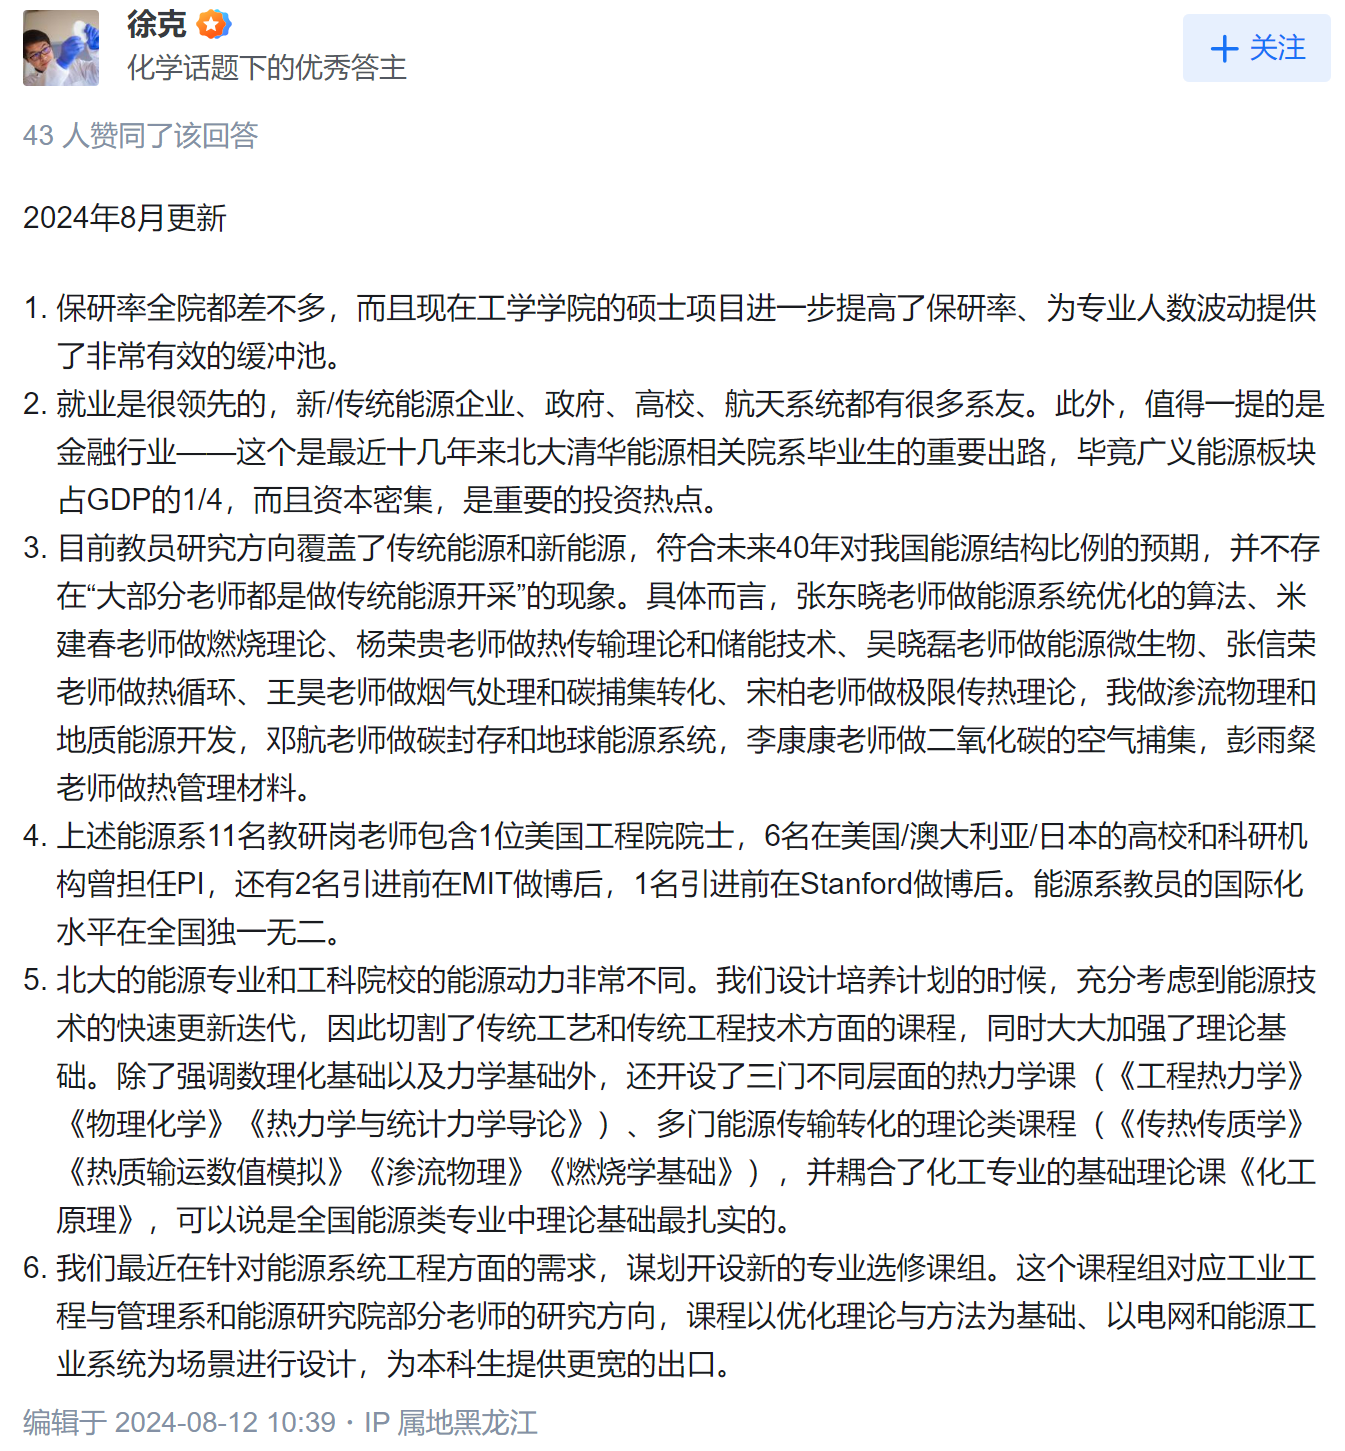
\includegraphics[width=0.7\linewidth]{assets/1.3.3徐克老师问答.png}
	\renewcommand{\figurename}{图}
	\caption{徐克老师知乎回答}
	\label{fig:enter-label}
\end{figure}

转自能源系徐克老师知乎回答。恰如陈正老师在树洞5G冲浪一样，能源系的徐克老师活跃在知乎一线。徐克老师对保研、就业、老师科研方向、课程设置等都进行了较为详细的讲述，同学们可以重点关注第3点。

来源：https://www.zhihu.com/question/583497117

\vspace{10pt}

\textbf{二、能源专业学习内容}

1. 非工学院（体育、通识、政治、英语）课程。

对于能源系的同学们来说，由于本专业课程难度相较理力等专业课程难度低，同学们可以有更多时间学习感兴趣的通识类课程。建议提前在树洞、课程测评等网站善用搜索，尽量不要选择给分迷惑、投入大于回报的课程即可。

\vspace{10pt}

2. 基础必修课

\begin{itemize}
	\item 数理基础课程：数学分析一、二(非强基同学可用高等数学B上下替换)、线性代数与几何、概率与数理统计、普通物理ⅠⅡ、普通化学B、（常微分方程）、（工程数学）……
	
	\item 力学类课程：工程流体力学、（理论力学B）、（材料力学B）、……
	
	\item 计算机基础课程：计算概论、数据结构与算法、计算方法……
	
\end{itemize}

括号标注的课程对于工科试验班（非强基）的同学是建议的自主选修课程，对于强基的同学是专业核心课（必修）。

\vspace{10pt}

大部分基础课程都会在前三个学期完成，对于能源专业来说，在培养方案上减少了部分数学课程，部分课程难度相较理力等专业降低，如用工程流体力学替换了流体力学。因为强基同学必须以理论力学为主修专业，所以理力专业部分核心课程仍是必不可少的。

\vspace{10pt}

这里需要注意的是开设在大一下学期的普通化学B和高等代数两门课程。由于在第二学期结束时才会选择专业方向，而部分专业要求必修普化B，部分专业要求必修高代，可能会需要在大二、大三之后补选相关课程。对于确定选择能源专业的同学来说，在大一时可以选择不修难度较大的高等代数。

\vspace{10pt}

虽然常微分方程、工程数学不是能源专业同学必修课，但在后续的学习中，相关课程知识还是会被用到。比如在工程流体力学中就会涉及求解常微分方程、以及工程数学中的复函数等。

\vspace{10pt}

3. 专业核心课
\begin{itemize}
	\item 热力学课程：工程热力学、传热传质学、热统导论……
	
	\item 能源传输转化类：传热传质学、热质输运模拟……
	
\end{itemize}


能源系专业课相对难度较低，易于理解，大多是基于热学、力学之上的课程，部分涉及化学中的热力学内容，如吉布斯自由能、熵、焓等相关概念。请大家相信有努力就会有回报。

\vspace{10pt}

4. 能源专业特色课程

这部分主要列举一些个人认为能源系在培养方案中比较有独特性的专业课。

\begin{itemize}
	\item 能源与环境系统工程导论（能环导）。这门课是能源专业大二上学期开设的专业基础课程，类似于工学院在大一上学期开设的现代工学通论。2023年秋季由邓航老师开设。课程前半学期主要由邓航老师讲解环境保护与修复、后半学期由能源系多个老师以讲座的形式讲解能源和资源的开发、生产、应用，老师大多会结合自己目前研究的方向课题进行介绍，是了解老师，选择自己感兴趣方向的机会。
	
	\item 金工实习。这门课程是由材料学院开设于暑期的能源专业必修课程。会安排去昌平校区住5天左右，住宿环境很好，课程给分很好，涉及车床加工、3D打印等多项具体的加工技术操作，是一门很好的工程生产实践体验课。
	
	\item 本科生实践大课堂。这门课是能源系面向大三年级开设的科研实践类课程，可以说是能源系自己的本研\footnote{指本科生科研。本手册后续内容对此有进一步介绍}。在第一节课会有多位老师介绍自己的项目供同学们选择，除了能源系自己的老师外，还有工管、先机、材料专业做与能源方向有关的老师。学期中主要跟随相应老师进行科研实践，期末以答辩汇报的形式完成。
	
\end{itemize}

\textbf{三、专业未来}

大部分同学主要的选择都是升学科研。能源系提供了很好的本科生科研环境，有利于同学们在本科阶段找到自己希望在研究生阶段继续学习研究的方向。此外，能源系大部分老师都有海外科研背景，国际化水平高，对于希望申请出国留学的同学来说，也有一定的帮助。

\vspace{10pt}

\textbf{四、学习体会}

1. 培养方案注重理论基础，学习过程注重工程实践。

能源专业是一门工程类专业。但在工学院整体注重数理基础、能源技术更新速度快的影响下，北大能源系的培养方案切割了传统的工程技术、更加注重理论类课程，而工程实践类的技能则是在鼓励同学们参与到老师的科研课题中学习的。

\vspace{10pt}

2. 以兴趣为导向的自我探索，非常nice的师生氛围。

能源专业课内学习相对不卷，但可能随着专业人数逐渐增加有所变化，同学们可以将更多精力放在本科生科研上或其他自己更感兴趣的领域。能源系经常组织一些师生聚餐、学长学姐本研升学经验分享等交流活动，帮助大家多次、详细地了解老师们的研究课题，找到自己感兴趣的方向。除此之外，每学期还会有班主任、辅导员交流聊天环节、期末考试学生宿舍走访慰问等等，及时解决同学们学习生活中的困难。

\subsection{航空航天工程}
\subsubsection{（1）2021级\ 柴宇澳}

北大航空系主要以理论研究为主，注重理论基础，可以算是力学专业的延伸。近年来航空系不断发展壮大，主要体现在：陈正老师转入航空系；连续多位教师入职；学生选择人数上升。主要的研究方向有：燃烧与航空发动机设计、流体力学、气动声学、一般力学等。航空系一些基础课程与理力要求相同（如高等动力学、材料力学等），增添一些航空航天相关课程（空气动力学、航空航天概论等），也会较理力少一些理论课（如固体力学等）。总而言之，难度比理力较低，但是内容很多都与理力（尤其是流体力学）相关。

\vspace{10pt}

航空航天工程系前景广阔，一是在航空航天科研院所工作（航天三院、五院、九所......很多很多）；二是在国企、私企工作（大疆（无人机相关）、华为（燃烧与电池相关）、美的（流动控制与湍流相关）等）；三是出国深造，后续在高校任职。

\vspace{10pt}

从我个人的学习体会来看，航空系的课业压力比理力小一些，相比于其他专业也不卷。航空系有许多优秀又有趣的老师：在空气动力学课上，吕本帅老师送给我了一架飞机模型，吕老师还带我们去参观航空航天博物馆；在航空航天工业实习课程上，周超老师带我们去密云放飞航模与无人机。陈正、黄迅、刘才山、李存标、程承旗、史一蓬等老师都是在各个领域登峰造极的教授。同时，在保研方面，航空系的老师更加愿意接受来自北大的本科生，航空系的保研率也因此非常高。不过航空系出国这方面可能会有签证上的困难\footnote{针对美国高校而言}，需要仔细衡量。个人感觉在航空系就读体验良好，氛围融洽，同学们相互学习，也不会盲目攀比内卷，就业选择也相对较多，适合对航空航天、流体力学等有兴趣的同学选择。

\subsubsection{（2）2022级\ 鞠志翔}

航空航天工程是和理论与应用力学比较相似的一个方向，在本科培养上削减了一些理论性较强的课程，如高等代数、弹性力学、数学分析三，以及将一些课程压缩学时偏重应用来讲，如数学物理方法上下压缩为工程数学，流体力学上下以工程流体力学替代等等。此外，有一些航空航天特色的课程，主要是工程热力学、飞行器设计与动力、飞行器结构力学、空气动力学基础。在升学上，既可以考虑航空航天的导师，也可以考虑理力的导师，如果是后者建议多学习（不一定选课）一些理力的课程，以应对夏令营的面试。

\vspace{10pt}

在航空航天工程专业本科培养方案中，除去计算机基础课、通选课、体育课、思政课、英语课等全校必修课程以及自主选修课程，专业课主要分为基础专业课、专业核心课和专业选修课三类。其中，基础专业课包括数学分析、线性代数与几何、普通物理。专业核心课为材料力学（及实验）、理论力学、高等动力学、飞行器结构力学、工程流体力学这种力学课，以及工程热力学、飞行器设计与动力两门主要涉及热力学的课，还有一门电子电路课和工程性较强但难度不大的空气动力学基础。专业选修课中有三门是必修的数学课，它们是常微分方程、工程数学和概率与数理统计；其他课程按照学分要求选课即可，其中计算方法、控制理论基础（自动控制原理）是相对用处较大的；工程制图个人感觉对后续学习基本没有帮助且任务量大；普通化学(B)和普通物理类似讲的杂但容易刷分，但对后续学习帮助也不大；航空航天工业实习非常水，可凑学分。

\vspace{10pt}

建议学弟学妹除去培养方案上的专业课，适当选修或旁听一些课程，比如数学分析三、高等代数、信号与系统等可以填补知识漏洞的课，举例来说，航空航天工程的培养方案只有数学分析一与二，缺乏级数的学习，此外工程数学也不会细讲傅立叶变换，而信号与系统会详细讲解。

\vspace{10pt}

下面根据几门个人选过以及印象较深刻的课程，向同学们分享一些具体课程的心得体会，希望可以帮助大家提升学习体验，其中基础专业课在此略过，线性代数与几何、普通物理一二以及常微分方程的笔记放置于北大网盘（见文末）中，可供同学们参考。此外，查看树洞中的课程测评也会给大家带来一些收获。

\vspace{10pt}

（1）电子与电路\ 黄迅老师 

评分机制：30实验 + 30开卷期中 + 40开卷期末

作业不计分。按照原始总分的排名给分，100到85一名次一分，85以下会有调整，给分很好。

\vspace{10pt}

上课建议认真听，中文掺杂英文，老师考点都会在课上说；课本是英文，考试可以带。课本建议按要求看完弄懂，其实干货不多。期中很靠后，基本是期末的预演。期末大部分会考期中原题，考完期中建议和同学把答案对出来。不建议考前突击。实验课为在面包板连接电路，并下载一些电路模拟软件，扣分不多。

\vspace{10pt}

（2）工程热力学\ 张信荣老师

评分机制：20作业 + 30大作业设计 + 50期末

如果不想选航系开的工程热力学，张信荣老师的课是个不错的选择。这门课课堂听感一般，会点名但不要求考勤，因此适合考前突击。期中设计超临界流体火箭发动机，认真写报告即可。期末偏重概念的考查，填空和简答占大部分，老师课上会讲一些例题计算题，期末大概率会考计算原题，给分很好。

\vspace{10pt}

（3）空气动力学基础 吕本帅老师
评分机制：25期中 + 35期末 + 40平时分，包括一个大作业

\vspace{10pt}

这门课程很多知识在工程流体力学和工程热力学中已经学习过，比如等熵流动、不可压无旋平面流动复势这些知识。新增加了一些结论性的知识，绝大部分计算都可通过查表代替公式计算，因此可以期末前突击记结论。

\vspace{10pt}

最后感谢观看，在本科学习过程中的一些学习资料已经放在网盘：

https://disk.pku.edu.cn/link/AA1EA6B17FBAC44A65AAF79260DB132729
中，大家可以参考。最后祝各位学弟学妹在燕园学业顺利，生活愉快！

\subsection{生物医学工程}
\subsubsection{（1）2022级\ 范文琳}

生物医学工程是一个所含内容非常广泛的专业，几乎任何涉及生物或医学问题的工程类实践都可以被划进这个范畴。因此，相比于具体知识的传授，生医系的专业课更加注重项目式的学习，并且会对一些科研和工作上的“软”技能有一定的侧重，比如小组合作、presentation、文书撰写等。生医系比较有特色的课程是系列PBL课程（i.e.生物医学工程原理、生物医学工程设计）。在这些课程中，老师会要求同学们以小组为单位，在一个学期内完成一个课题的文献研究，或实现一个小型项目。过程中同学们可以向任何可以得到的资源寻求帮助，主管课程的李长辉老师也会为各组提供一些如何求助的指导与建议。

\vspace{10pt}

科研方面，生医系对于本科生提早进行科研实践给予极大的鼓励。生物医学工程专业对口的老师很多，但具体的研究方向之间也相去甚远，包括成像、计算、电子，也有偏向纯生物的课题组。大家可以在未来技术学院官网上查看老师们的研究方向，通过和老师约谈或者听组会的方式来决定自己更加感兴趣的方向。一般而言，大家会在确定自己的方向之后在选课上进行一些调整，以规避交叉学科学习中通常存在的“博而不精”的问题。

\vspace{10pt}

另外值得注意的是，尽管生医系的强基生被要求修一系列力学系课程，但这些课程在难度要求上和正统的力学系课程还是有一定的区分。当然，任何理工类学科中数理基础总是重要的，诸君可以自己多多留意（x）。

\subsubsection{（2）2022级\ 李昆泰}
\textbf{生物医学工程系概况：}

生物医学工程系（常简称生医系，后文亦沿用，这个名字可能小有误导性，之后会在文章中详述）和材料系是工学院“系”、“专业”或“方向”中较为特别的两个，因为实际上生医系和材料系的“研究生院”都是单独成院的，它们对应的学院分别是未来技术学院和材料学院。未来技术学院这个学院可能在大家看来相当“科幻”，觉得我们搞的好像是什么天顶星科技一样。在某种意义上确实，我个人也觉得我们在创造一些极为有意义的工程发明和科学发现。更实际地说，北大的未来技术学院面向的就是未来的生命健康，所以也无怪乎生物医学工程系是在未来技术学院中的一个系了。简单理解的话，生医系是未来技术学院的一个系，而这个系的本科生放在了工学院这个学院中进行培养。大家如果选择国内深造，大概率可能会选择进入到未来技术学院的课题组中。

\vspace{10pt}

\textbf{生医系的入学渠道和同学构成：}

生物医学工程系现在应该有三个入学渠道。一是高考裸分录取中的“工科试验班”类，二是强基计划力学类的“理论与应用力学（生物医学工程方向）”，三是强基计划生物类的“生物四”。其实在大一选专业后，实际进入生医系就读时没什么差别（生物IV我现在不清楚），编班都在生医班，成绩排名、评奖评优什么的都在一起排，也享有同等的进实验室等的资源。差别主要在培养方案上：强基需要比非强基的同学多修一些力学类课程，数学类课程的难度要求可能也会高一些；非强基的同学则需要修读更多学分的生医工专业相关的课程。

\vspace{10pt}

\textbf{生医系在做什么：}

前文说了，生医系是未来技术学院的一个系；同时，生医系还是未来技术学院唯一的一个系。大家未来路径选择上很大的一个优势就是——本科从生医系毕业，研究生可以选择整个未来技术学院的方向\footnote{当然也可以选择如生科、人工智能等其它学院的方向，这里讨论的是主流的选择}。所以，与其说是在讨论生医系在做什么，其实更多讨论的是未来技术学院整体在做什么，乃至整个生物—医学—工程领域的交叉点上大家在做什么。

\vspace{10pt}

先从“狭义”的生医系本身讲起。这里要澄清一个长久以来的误解：生医生医，其实是生医工这个“生物医学工程”的简称的简称，“生”和“医”是工作面向的核心问题和应用场景，“工”则是这个专业的“技能”核心。大家可能会认为生医系是做生物科学研究的？还是当医生的？进检验科的？等等等等，其实都不甚准确，或者说不是标准的路径。准确地说，生医系可以说是给生物科学研究造更好的仪器设备，让科学家看得更清楚，操作得更“稳准狠”，打开更多的研究可能性的工作；是给医生创造更好的医疗器械和临床工具，或者给患者本身制造更好的健康检测、干预与辅助设备，增进病人的生存率和福祉，为更多疾病带来创新型的治疗与干预方法的工作。它的学科基础主要是工程学和物理、化学、生物学；关注的是解决生物科研和医疗临床问题\footnote{北大生医系前者做的较多，但社会上主要谈的是后者}；而在未来，它更有可能带来大幅长寿、人机融合等人类社会的重大变革。

\vspace{10pt}

在临床领域，生医工所做的可以看到的工作已经非常丰富了。大到CT、磁共振、超声等各种医疗器械，小到血压计、血糖仪、血氧仪等日用医疗健康产品，再到嵌入到智能手表里的心率检测等功能，都是生医系（与其他学科交叉融合）的创造。脂质体药物、CAR-T等创新疗法其实也可以称之为一种“针对生物的面向医学需求的工程学”，所以这个学科有相当的学科交叉性和知识结构多样性。进一步的，在“广义”的生物-医学-工程领域上说，我们会在各个尺度、各个物理原理上进行创新。我们会利用力、热、光、电、声等物理原理，酶促反应动力学等化学原理和激素调节等生物学原理，一方面探测生物从分子细胞到个体群体的各种信息，另一方面用这些自然的力量去扰动、调节乃至控制生物系统，以增进对生物系统的理解和对人类调控生物系统的手段的掌握；另一方面，我们会从物理的疆域跨越到信息的疆域，利用算法、大数据与人工智能的力量对我们获得的信息与能力进行更强大的总结、提炼与应用。这些抽象的理念具体化到各种方向中，就是生物成像\footnote{利用光学获取细胞及亚细胞尺度的信息}、生物力学\footnote{工学院可能做的比较多，提取生物学现象中所蕴含或利用的力学规律}、神经电生理和神经工程\footnote{通过电信号收集生物体的信息和对生物体进行扰动或控制}、生物传感器与生物电子学\footnote{利用电子元器件构建对不同物理信息的提取装置}、生物探针\footnote{利用蛋白质等生物分子的相互作用原理与光学等物理原理实现对生物系统的观测}等等。

\vspace{10pt}

未来技术学院还有分子医学所、国家生物医学成像科学中心、大数据与医学人工智能系等机构，其研究方向其实也在我刚刚讨论的广义生物—医学—工程交叉领域之中。相关的研究方向和实验室也是大家可以去尝试、选择的。在真正的科研实践当中，尤其是生物—医学—工程这个大的领域之中，科学与工程、发现与发明、研究与创造、提炼与综合一直是相互交织、相生相荣的关系。我们很难划出一个到底什么是生物科研，什么是生物医学工程，什么是分子医学研究的分界。但只要大家对生物学问题、医学问题和针对二者的工程问题中的其中一点有所兴趣，都欢迎大家来到生物医学工程这个广大而充满无限可能的领域中探索与创造。

\subsubsection{（3）2022级\ 丁奕航}

生医工专业近几年的变动比较大。作为22级的本科老登，我的分享主要基于自己力学强基的身份，兼有对非强基培养方案的一定了解。对于26级生物强基的同学，可能只在部分方面有参考意义（叠个甲先）。

\vspace{10pt}

生医工专业是一个非常广泛的专业。广义地说，任何在生物或医学方面的工程相关课题都属于生医工专业。北大的生医工内部也分为多个方向，主要包括分子细胞、成像、生物计算、生物材料等，每个方向都各有特色。由于强交叉的学科特性，往往每个方向所需要的专业能力都是多样而不同的。因此，建议同学们从大一开始就多多了解各个方向的具体情况，大致包括这个方向在做什么事、有哪些老师在研究哪些具体项目、可能需要哪些知识技能、自己是否感兴趣等。这一过程不必着急，通过专业课的学习、与老师同学们的交流、校内的各种讲座课程和官网上的教授主页等慢慢熟悉即可，主要是为了明确自己的兴趣方向。

\vspace{10pt}

生医工专业本科期间的学习和科研是紧密结合的。由于专业内各个方向区别较大，培养方案内的课程难以深入每个方向，更多是普遍地教授一些初级技能，给同学们一个初步认识。因此，大家往往需要在明确一个兴趣方向后尽早地进入老师的课题组，通过读论文、跟项目等方式，在应用中学习具体的实验操作、软件使用和更为细致的生物医学和数理力学知识，将其与课内学习相结合。这样的模式一方面需要大家一定的自学能力，另一方面可能也需要大家权衡课内外学习，放弃一部分课的优绩，换得更实用的技能。关于学习部分，还想多劝大家不要过分重视绩点，在专业人数持续增长的过程中不要被焦虑裹挟去卷一些没必要的事，而是为自己找到适合的方向，由兴趣和实用需求驱动，放松心态去锻炼一些自己需要的能力。即便是从功利角度出发，在保研和留学中绩点也并非第一指标，只是一个够用即可的门槛。学习能力、科研经历、乃至于合作能力、人际交往能力和性格等软性特点才是老师们更看重的。

\vspace{10pt}

在生医专业的学习中，还需要注意根据不同学科课程的特性调整自己的学习方式和习惯。我们的培养方案要涉及数理化生医等多种课程，其中数理（力学）课更注重理解推理，而化生医学课往往需要更多的记忆。用适合一种课程的习惯去学另一种课可能会吃亏，一定要注意避坑。（说来都是辛酸泪）

\vspace{10pt}

关于保研，第一当然是及早联系老师，在大三暑假前尽量有一点点实在的科研经历。这主要是因为夏令营时科研经历是最主要的考察项目，老师可能会问一些较为深入的问题，科研水不水一问便知。第二是建议多方面了解，不要仅限于未院，校内叉院、生科乃至信科等院系的一些项目都可以尝试，非强基的同学也可以联系外校老师们\footnote{如果政策没有变化的话}。第三是不要太在意沉没成本，当你觉得自己和当下的课题组不合适，直接换就好，毕竟直博是五年的相处，比很多恋爱都长，还不能轻易分。关于出国本人不甚了解，不过在本科低年级需要做的事相差不大，在此就不赘述。

\vspace{10pt}

最后，祝愿大家在工院快速扩张内卷加剧的当下，还能始终保持初入燕园的这种兴奋、好奇与探索欲，在这多彩的校园和有趣的专业里，享受短暂而美好的大学时光。

\subsubsection{（4）一位希望保持匿名的同学}

个人主要参与以实验为主的方向，且非强基，所以力学课学得比较少，以下讨论都基于这个前提展开（首先叠甲）。

\vspace{10pt}

\textbf{关于方向：}

我了解的实验室大多与生科方向较为接近，但整体而言更偏向临床应用，个人认为在科研中属于比较容易找到获得感与方向感的方向。实际参与过程中的主要感受是，这类动手较多的实验，仅仅在课本上学习或是在网上看视频，和自己亲自去参与一个完整的实验流程所感受到的是非常不同的，想了解相关方向的话也许可以早点去实验室了解一下，而且上手做过后也会更容易理解相关论文的研究方法等。

\vspace{10pt}

\textbf{关于上课：}

由于本人是高数B + 医预有机B选手，这两年的深刻教训就是基础课需要亿点练习，和分子细胞、生理学这样“会背=会做”的课不太一样，这些基础课的考试由于题目不少+难度不算特别高+不调分，所以几乎每一分都是要靠平时的努力和汗水自己做出来的（悲），仅仅理解完全不练习可能直接导致在交卷前对着会做但来不及写的题目发出尖锐的爆鸣，不过相信小灯们带着刚从高中训练出来的新鲜大脑，还是能轻松应对的（确信）。

\vspace{10pt}

最后夹带一些私货，推荐几个也许不是必修但有意思的课程\footnote{“有趣”的评价出于个人喜好，可能对一些未来倾向不同研究方向的同学来说比较无聊，另外尽管开课老师都非常nice但没有水课}。

\vspace{10pt}

（1）sky\footnote{即“生科院”的首字母}杨竞老师的免疫学。个人觉得老师讲课很有意思！虽然受限于课时很多细节没办法在课程中全部覆盖到，但作为入门了解感觉很不错；

\vspace{10pt}

（2）孙红芳老师的生物医学工程综合实验。我以前没学过生物竞赛，在该课程中可以学习到科研常用的实验操作及原理，并且练习一项很重要的技能——自己看protocol学习新实验的操作；

\vspace{10pt}

（3）胡薇薇等老师开设的文献写作与报告。虽然是通识课，但正如胡老师在开课时所说，这门课或许在通识课里有一点“硬”，但能坚持下来的同学一定收获满满，个人认为能经过几周甚至一两个月的准备，精读一篇论文，从其研究背景到方法、结论，流畅地作一次模拟学术汇报，可以对自己感兴趣的研究方向有更深入的了解并且锻炼一下学工科后日渐贫瘠的表达能力，很有成就感（还弥补了本人组会第一次讲journal时磕磕巴巴的遗憾hhh），并且听听其他不同专业同学的汇报，还是挺有意思的。

\subsection{材料科学与工程}
\subsubsection{（1）2021级\ 李一川}
材料专业学习的知识会涉及更多的领域，包括物理、化学、生物等多个方面的知识，课程内容也比较丰富。同时，在注重基础知识学习之上，会更加强调与实际应用和生产生活相结合。课程讲述的内容也非常前沿，许多也是当前社会发展的热点话题，比如钙钛矿半导体、新能源电池、柔性电子等等。材料学院目前已经单独成立学院，导师数量众多，涵盖的研究范围也非常的广，对接资源非常丰富，同学们可以根据自己的兴趣，非常自由的选择导师加入课题组进行本科生科研训练。

\vspace{10pt}

材料专业的本科教育更加强调基础知识的学习，以及大量细分领域的了解，拓宽知识面，而大部分同学会选择在本科毕业后继续在某一个专业领域继续深造，攻读硕士或博士。

\subsubsection{（2）2022级\ 曾帅鹏程}
\textbf{关于基础课程：}

1. 全校通选：全校学生情况都差不多，但作为工院学生尤其会对三四类通识感兴趣，所以务必注意一二类通识选择时一定要选核心通识课，避免多修。

\vspace{10pt}

2. 工院基础：以数分、高代等专业课程为代表，在大一未分流时，全体学生情况统一（强基与非强基会略有不同，具体请研究培养方案）。值得注意的是，工学院对数理的要求较其他理科学院来说有过之而无不及，且范围广（计算机、数学、物理、化学都有涵盖），务必对此多加上心。若对材料专业感兴趣，建议大一下修完大学化学，减少之后学期负担。

\vspace{10pt}

3. 材料专选：在大一后分流来到材料专业，需要修习许多专业课程，强基生不能完全丢掉理论力学的学习，因此课程任务量会比大一学年加重。理论力学方向相关课程会和生医、能源一起开班上课，难度略低但也不可轻率。材料方向课程则以小班授课形式进行，代表课程有：材料科学基础、材料物理、物理化学、材料学中的量子与统计……这些课程理论性极强，会结合当前材料方向前沿进行讲解，内容在化学基础比化院较弱的情况下会显得晦涩难懂，但很有必要花费大力气进行深度学习。工学院的课程课后花费时间一直位于北大第一，希望同学们早做心理准备，但也要相信，只要肯下功夫，成绩也不会辜负你的努力。

\vspace{10pt}

4. 自主选修：这方面课程需要和你的研究方向相结合，材料学的知识十分广博，在确定好自己今后学习方向后特异性极大，结合方向多修习校内相关课程，方能使学业一帆风顺。

\vspace{10pt}

\textbf{专业未来：}

材料学本科就业不占优势\footnote{其实除去金融和计算机，很少有专业会愿意本科后就业}，在读完研后\footnote{听说本校通常给博}就业方向极广。材料学科囊括范围极多，从本校导师研究方向便可管中窥豹：肿瘤疫苗、电催化、锂电池、纤维、钙钛矿、高分子等。所以需要尽早确定从事材料科研的方向，毕竟任何一个方向都需要精深学习，都需要花费时间。在研究生毕业后有许多出路：博后发展、企业研发、高校任职、科研所任职等。具体内容都是因人而异。

\vspace{10pt}

\textbf{学习体会：}

在化学基础较化院薄弱的情况下，每一门材料的课程都会显得晦涩难懂，每一门专业课程都需要在课后投入大量时间进行学习。但要相信，每一分努力都会带来回报。材料专业对科学前沿的了解十分重要，所以了解自己方向的科学前沿发展情形都很有必要，需要自己课后花费时间进行了解。

\subsubsection{（3）2023级\ 惠炜博}

\textbf{关于课程学习}

材料专业与其他传统力学类专业很大的区别是，在分流之后的第一年就会将学习范围极度拓宽，数学、物理、化学和更加交叉的方向都有所涉及，我本人是工科试验班类（非强基），对这种变化的体会尤为深刻。当然这也意味着在选择材料专业之后有了一次重塑的机会：课程不那么依赖大一数理课的基础，继续付出努力仍然有可能在材料专业闪闪发光。

\vspace{10pt}

由于工学院本科生的化学基础较弱（此处是对非化学强基的同学而言），在上材料专业的核心课如：材料科学基础、材料物理、材料中的量子统计的同时，还需要在普通化学B的基础上学习物理化学、有机化学B、分析化学等课程，相当于是边打地基边造楼。尤其是物理化学中有很多重要的基础内容，却被放在大二下学期。不过各位也不必过分担心，与化院相比，我们所学的基础化学类课程已经是减学分、减学时、减内容之后的版本了。只要肯认真学习，还是能够满足考核要求和基本的知识体系构建需求的。此外，由于排课学期和排课顺序等因素，负责教授专业核心课的老师们可能会选择在自己所讲的部分向大家补充前置知识。在这里也建议各位想选择材料专业的同学们要培养充分的自主学习能力。

\vspace{10pt}

材料专业的课程（基础化学类课程除外）目前来说基本形成了一种范式，即课堂讲授＋小组文献汇报＋习题课（若有平时作业）＋闭卷考试，考查的能力也是多方面的。关于小组文献汇报，老师会给出一些和课程内容有关联的文献，同学们自己去选择自己感兴趣的文献进行研究和汇报，一般来说时间在20至25分钟。有的老师比较排斥对着稿子读或者是当PPT reader，所以这个部分需要很强的表达能力和变通能力。关于习题课，即老师或助教将具体的题目分配给具体的同学在特定的一节课来讲解自己的思考和解答过程，几乎没有选择空间，讲题的过程也非常考验表达。关于闭卷考试，材料专业核心课需要记忆的内容偏多（非常多），理解的东西也不少，比较考验记忆力和知识体系化的能力。

\vspace{10pt}

\textbf{关于就读体验}

尽管自己觉得不算轻松，但不得不承认，与工学院其他专业相比，材料专业的课程难度总体上较小。只要肯付出努力，稳扎稳打，基本都会取得比较不错的结果。此外，大部分老师会在上课时向同学们介绍自己的实验室所研究的课题方向，也很愿意跟同学们进行课间交流，让大家在官网之外能够有更加生动的了解。如果是像我一样的工科试验班同学，在大二时就可以免于上很多3学分4学时的课，留出更多的学习时间去做其他事情，例如了解老师、旁听组会、进实验室做本研等。外界（甚至我们自己）经常调侃“生化环材”是四大“天坑”，但其实翻看材料专业老师们的主页就会发现，他们从事的大部分都是迎合新时代国家发展战略需求的研究。大部分材料专业的同学会选择本科结束之后再读研究生，而在材料专业的保研压力也相比其他专业要小很多。

\subsection{机器人工程}
\subsubsection{（1）2021级\ 刘家豪}
\textbf{专业内容}

从本专业的必修课设置看，机器人系统的设计、制造中所涉及的各环节内容均有覆盖，课程涵盖集成电路、控制器、机械设计、建模等内容。个人认为通过本科阶段的学习，了解制作完整的机器人所需知识，掌握MATLAB、SolidWorks等常用软件的使用，甚至自己DIY一些简单的机器人应不成问题。在专业必修课的主线之外，亦有较为丰富的选修课程可供体验，譬如机器学习、嵌入式、图论、计算机视觉等相关课程。

\vspace{10pt}

总体来看，作为一个多学科交叉的本科专业，机器人工程的课程设置更注重广度，培养能力全面的人才。建议结合本科课程的学习、实验课体验、本研经历选择自己感兴趣的具体研究方向。如果对机器人领域感兴趣的话，相信本专业能够给你良好的学习体验。

\vspace{10pt}

\textbf{自身体会}

就我个人三年来的学习体验而言，与其他工科院校的类似专业相比，本专业也较为注重数理基础的培养，这也是本校工学院的院系特色之一，具体体现为大一需要完成多门基础数学课的学习，后续也有较多数学类课程可供选择。学有余力的同学可以尝试本院的“理力+机器人”双主修项目。

\vspace{10pt}

若要达到精通某一具体的机器人领域，以作为将来科研或就业道路的立身之本，我认为仅完成本科阶段的课程学习可能并不足够，课外的自学和实践也很重要。本科学习期间适当参与科研项目或竞赛更有助于自身技能的完善，如大二下学期报名参与自己感兴趣的本科生科研项目等。

\vspace{10pt}

\textbf{未来去向}

若想继续从事机器人领域，相比与直接本科就业，我个人认为读研深造可能是更为合适的选择。下面我就我个人的了解大致介绍与本专业相关度较高的科研方向。由于本专业涵盖较多学科的内容，相关可供选择的科研方向亦丰富多样，在此仅举一些我较熟悉的例子。例如从事某一细分领域的研究，以机器人感知为例，硬件如视觉、触觉传感器等的设计，软件如多传感器融合算法、SLAM等，都是可选的方向；又如完整机器人系统的设计，譬如特定用途的机器人如某一类医用机器人、水下机器人、软体机器人等；将AI与机器人融合也是时下较为热门的方向。另外，进入工学院官网浏览本系老师的研究方向或咨询学长学姐等，或许能让你对本专业的科研方向有一个较为全面的认知。

\vspace{10pt}

我个人对于本科就业了解不多，在此也就不过多介绍。进入相关科研院所工作、加入科技公司或某些大厂的机器人研发部门，一般是较为对口的选择。当然，有了北大计算机通识课、专业相关课程所积累的编程基础，进入互联网企业工作也不失为一个选择。倾向于就业的同学可以多多留意院系宣讲时介绍的毕业去向统计或咨询学工办老师。

\subsubsection{（2）一位希望保持匿名的同学}
机器人工程专业涉及多个领域的基础课程，包括力学（理论力学、高等动力学）、数学（高等代数、常微分方程）、电路（如数电、模电）、机械（如机械设计基础、机器人学概论）、自动控制原理等。这些课程是入门的基本要求，也是未来深入学习和研究应用更具体内容的基础，需要大家都能有一定程度的掌握。因此，对于想要选择机器人专业的同学来说，前两年的首要任务就是重视这些基础课程的学习。

\vspace{10pt}

除了基础课程的学习，第二个关键任务是主动探索本专业的研究方向。机器人专业涵盖了多个研究方向，包括智能系统与控制、群体博弈与智能决策、医用机器人、水下机器人与装备、先进制造与工业软件、无人系统的自主决策与规划等\footnote{大家可以到工学院官网查看更具体的内容}。建议大家积极利用各种机会，如现代工学通论课程、各类讲座，以及与老师的交流，去更加深入地了解每个方向的研究内容。在还没有明确的兴趣时，多与老师交流将大有裨益。在对各个研究方向有了一定了解后，就可以选择一个合适的时机，主动联系老师，参与一些本研任务。最初可能有忐忑和顾虑，但是这种边学边用的学习模式，给予我们很大的成长进步的空间，不仅能够加深对知识的理解，还能提升解决实际问题的能力，最重要的是也能检验我们是否真正感兴趣\footnote{如果发现自己实在不感兴趣，那么就去探索下一个方向，试错空间很大的！}，这对我们的自身发展能起到更全面的帮助。

\vspace{10pt}

此外，在后续的课程学习和本研中，MATLAB、Python以及SolidWorks等软件将会频繁使用。因此，建议大家提前自主学习+练习这些工具的基本操作内容\footnote{迟早都需要自学的}。

\vspace{10pt}

希望大家在选专业这方面上不会有太多的困惑啦，如果有，那就及时主动寻求帮助！愿大家能够享受这段美好的时光！

\subsubsection{（3）2022级\ 欧阳卓}
\textbf{专业学习：}

在专业必修课中，首先最基础也是最重要的是一些数学物理和力学的课程，俗话说“像科学家一样思考问题，像工程师一样解决问题”，这些基础课程可以让你对基本的理论体系有一个初步的了解，搭建起自己脑中的“科学大厦”。进一步是关于机器人相关的专业课程，以我的理解可以大致分为三层：

\vspace{10pt}

底层设计：

对于机器人，底层的机械结构是机器人的骨架，我们可以通过例如机械设计基础、先进制造基础等课程了解机械结构设计的方法、机械的加工制造等方面的知识，并学习诸如工程 CAD、SolidWorks 等软件的使用方法；

\vspace{10pt}

“血肉”铸造：

电子电路、单片机、传感器相关电子元件好比机器人的血肉，它们将底层机械结构有机地结合起来，使得机械臂能动起来、机器人能像人一样“看见”外部信息，通过模电、数电、机器人学实验二等课程可以对电子相关内容有个大致的了解；

\vspace{10pt}

“大脑”控制：

对于机器人来说，顶层的算法、规划、控制等内容就像机器人的大脑，当机器人通过传感器得到相关指令后，大脑会对这些指令进行处理，并告诉机器人下一步该怎么做、怎么将信号转换为动作并实现。这一部分涉及内容较广，可以通过一些计算机算法相关的课程和控制等相关课程来学习。

\vspace{10pt}

上述三部分内容仅仅是我的个人见解。以我个人而言，我会通过专业必修和选修课对各个部分进行一个初步的了解，然后会对自己感兴趣的方向进行更广泛、更深入的了解。比如我对机械不是很感兴趣，但会继续选一些微电子、机器学习、强化学习的课程，对电子和算法层面有更多了解。

\vspace{10pt}

\textbf{科研方向：}
机器人可选择的科研方向很广。你可以尝试机械的项目，进行一些机器人实物的设计；也可以进行嵌入式开发、对电子电路进行深入的探索；同样也可以进行优化控制的研究。进组也会拥有更多元的选择。我在大二时，就是先加入了智能学院王弈森老师组进行机器学习的研究。大二下也旁听过机器人系李忠奎老师组，大三上加入了工管系尤鹏程老师组进行强化学习、优化控制等方向的研究。大家在选择科研方向的时候思路可以打开，不一定仅仅只局限在自己的专业领域，因为你会发现开始科研时很多知识你都得从头开始学，所以不要因为这个领域你不熟悉就气馁，更不要觉得自己专业对口就能很轻松地解决科研问题。

\vspace{10pt}

\textbf{个人体验：}
关于自身学习体验，这里我主要谈谈课内选课、学习等方面。

\vspace{10pt}

1. 关于选课，前面很多学长也谈到了，在这里我还想说一点我关于绩点\footnote{考虑到从2025级开始取消绩点制度，请大家将其看作是“成绩”的同义词}的认识。成绩的高低有很大一部分来自选课的规划，比如你选了一门好课，可能你比别人花更少的时间就能拿到更不错的分数。这样说可能有点功利，但对于较为看重成绩的同学来说，选课是你同样要花很多时间去规划的一件事，因为选择有时候比努力更重要。

\vspace{10pt}

2. 有的新同学可能会有很多东西想学，一学期一不小心就选了一大堆专业课和通选，想要挑战自己。以我的经验和个人见解，这样一来，可能会因为课业压力过大而心态爆炸，导致过早实现绩点自由\footnote{指绩点处于较低水平，产生“无所谓”的态度}（一学期八门十门专业课还能3.9+ 的大佬除外）。另外，很可能因为课程过多，你会把大量时间花在写作业、做lab和应付考试上。一学期学下来成绩不错，但回过头来发现很多东西只是浅尝辄止，并未深挖，学过了就忘了。第三，从我个人角度，上课并不是学习效率最高的方式，如果你有足够的自律（这个前提很重要！），你完全可以只学基本必修课，其他想学的课程都自行找资料学习，这样可以省去很多无用的作业、无用的内卷以及考前背诵一些犄角旮旯的东西的时间。但说实话，我觉得上课会通过作业、考试、绩点等方式逼迫你学习。如果没有课程的压力，自己又没有足够的动力（无论是热爱还是单纯的自律），时间可能就都用在摸鱼划水玩游戏上去了。最终知识没学会，学分也没混到（本人的惨痛经历 ×），故这一点因人而异。

\subsubsection{（4）2023级\ 石昊}

\textbf{专业理解：}

正如培养方案第一句话所说：“机器人工程专业是……涉及机械、电子、力学、计算机、自动控制、人工智能等众多学科。”工学院的机器人工程是一个涵盖学科非常多、学习内容非常广的专业。就拿课程设计来说，本科阶段需要修读的课程涵盖了机械、电子电路、力学和计算机等方面。同时，该专业也对学生技能的广度和深度提出了要求，包括但不限于计算机编程、SolidWorks建模、Arduino控制和PCB电路设计等。个人认为工学院机器人工程专业的课程设计比较合理，其涵盖了机器人领域最底层的知识体系和技能点。不过，鉴于专业的特性，不可避免地会因为学习的内容太多太杂而导致学生对日后的方向产生迷茫和焦虑。而且，不可否认的是，相较其他工科类院校学习机器人的同学，贵校\footnote{指北京大学。“贵校”是北大同学口中对北京大学的调侃称呼}机器人工程专业的同学在动手做项目或者做科研方面的经历会比较少。理论固然重要，但是作为一个工科学科，实践经验要比理论学习更重要。这个时候可能需要同学发挥主观能动性，积极寻找科研和项目的机会，比如联系导师进课题组和参加有关的机器人比赛等。

\vspace{10pt}

\textbf{就读体验：}

就我个人来说，在机器人专业的就读体验是很不错的，主要有以下几点。首先，正如前面所说，学院设置的课程体系全面涵盖了机器人领域的核心知识。同时，得益于北大自由的选课制度，如果对计算机、AI和电子这方面的知识有更深的需求的话，还可以选择信科的课程来完善自己的知识结构，也为个性化发展提供了广阔的空间。此外，机器人工程专业拥有开放包容的学术氛围。以我的切身体会为例，我经常和同专业同学及课题组成员展开深入交流，既探讨课程内容，也分享研究思路。这种思维的碰撞，不仅拓宽了我的专业视野，更显著提升了我的学习效率和科研创新能力。此外，作为工学院2019年设立的新兴学科，机器人系汇聚了一批十分优秀的青年教师。他们的加入为专业发展注入了强劲动力，使整个学科呈现出蓬勃发展的态势。这也让我个人觉得机器人系正生机勃勃，蒸蒸日上。

\vspace{10pt}

\textbf{给学弟学妹的话：}

我在前面也说到了，由于需要学习的内容太多太杂，很多同学可能会迷失方向，产生焦虑和不安的情绪。我认为尽早联系导师进组是个明智的选择。即便暂时不直接参与具体研究，单纯观察前沿科研人员的工作状态和研究内容也极具价值——正所谓“他山之石，可以攻玉”。学习和借鉴他人的创新成果，往往能帮助我们逐步沉淀出自己的研究方向。同时，在学习和科研过程中，积极与同学和老师交流往往会有意想不到的收获。我个人也正在寻找未来的方向，上面的话也谈不上建议，更多的是和学弟学妹们共勉。学弟学妹们刚步入大学校园，可能会感到焦虑和不适应。其实本科的试错成本是很低的，大家可以勇敢尝试自己感兴趣的一切事物。无论遇到什么困难，希望大家保持乐观，坚信一切都会越来越好。不管同学们之后是否会选择机器人专业，祝愿大家一切顺利，都能够找到自己喜欢的方向，日后能在自己的领域里发光发热！

\subsection{环境科学与工程}

\vspace{10pt}

\textbf{环境化学}


\subsubsection{（1）2022级\ 王成昊}

环境科学与工程学院主要包括四个专业方向：环境科学、环境工程、环境健康与环境管理。通过强基计划进入北大的同学修读的是环境化学专业，在后续研究生阶段才需要从以上四个方向中选择一个自己感兴趣的方向。环院老师的研究方向十分多元化，从大气物理、大气化学，到仪器开发、材料合成，再到生态学、微生物学，以及经济学、管理学、法学和伦理学都有涉及。具体的专业情况和老师研究方向，可以到学院官网的“师资力量”一栏查阅。需要额外指出的一点是，环境科学与环境工程这两个方向研究内容实际上有着一定的交叉与重叠，具体选择时更应关注导师的具体方向，不必拘泥于某一专业方向。在选择本研导师或者研究生阶段导师时，可以广泛地搜集老师们的资料，尤其是最近发表的文章，了解老师们目前感兴趣的方向。此外，也可主动约老师聊天或旁听组会，感受课题组氛围与工作重点。

\vspace{10pt}

环境学科作为一个问题导向性学科，其最终目的在于解决实际问题，因此课程设计上会比较“宽口径”。环境化学专业的课程大致分为三大模块：一是夯实数理基础的公共必修课，包括高等数学、线性代数、概率统计、计算概论等；二是建立化学根基的化学类必修与选修课，其中不少课程与化院专业课直接对接；三是旨在掌握环境专业知识的环境类必修与选修课。由于课程涉及范围较广，教学内容跨度较大，想要每门课程都追求完美不太现实，建议结合自身实际情况和未来发展方向综合考虑，合理分配投入到不同课程上的精力和时间。

\vspace{10pt}

关于选课，还有几点碎碎念。首先，切勿仅凭课程名字臆断课程内容。选课前最好看一下课程的教学大纲与安排，同时搜集一下这门课的往年评价，确认其确实符合自己的选课需求后再选课。其次，不必畏惧中期退课。如果在课程学习中压力过大，且期中成绩十分不理想，在确认后续有机会重新选课后，最好不要硬撑，果断退课，保住成绩方为上策。最后，需要强调自学能力的重要性。不同课程的授课风格不同，如果课程教学方法和进度不适合自己的节奏，一定程度上选择自学或许是一个不错的想法。此外，大学的学习也不必拘泥于课堂，本科生科研、学生工作、社会实践、社团活动、课外时间也都是学习的机会。

\vspace{10pt}

环境作为一门相对冷门的专业，每届都会转出不少同学，继续留在本院的同学大多会选择继续深造，也有少数选择直接就业。对于是否转专业这一问题，我认为转专业是非常正常而且合理的选择。但是转专业的前提是对转出和转入的专业有着比较充分的了解，同时有着较为明确的职业规划。专业各有利弊，找到既喜欢又适合的方向，是大学阶段最重要的一课。

\vspace{10pt}

最后，真诚欢迎各位同学加入环院大家庭！祝愿大家能够在大学四年间，感受大学的酸甜苦辣，寻得自己真正的热爱与理想，度过一段“五味俱全”的充实生活。

\subsubsection{（2）2022级\ 陶安然}

\textbf{（1）学习内容}

我们的专业课主要由环境科学与工程学院和化学与分子工程学院两个学院开设（以下简称“环院”和“化院”）。其中化院开设的课程主要有普通化学、定量分析化学、有机化学、物理化学和一些实验课程。相比于化院的学生，我们学习的化学课程难度低一些，对于有化学竞赛基础的同学来说，化学课程的学习是比较轻松的；没有化学竞赛基础的同学则要做好啃硬骨头的准备，但是认真学习也是可以学懂并且获得不错成绩的。环院开设的课程主要有环境问题、环境科学、环境监测、环境工程（一）（二）等，和非强基专业学生的基础环境课程比较一致。当然了，计算机基础课和基本的数学课也是我们要修读的，鉴于之前的部分数学课对同学们来说难度较大，学院对培养方案中的数学内容做了调整，希望大家能拥有一个良好的数学学习体验。

\vspace{10pt}

\textbf{（2）个人学习体会和建议}

环境化学的学习内容还是很有趣的。我觉得与其他专业较为不同的是，我们能将学习到的化学相关基础知识应用到具体环境问题上，从分子结构出发解释环境现象的机理。本人没有化学竞赛的基础，所以在刚刚入学时，学习普通化学这门课要付出比较大的时间精力。但根据身边统计学，是否有竞赛经历对大家后续的成绩和整体发展几乎没有影响，所以大家不用因为竞赛基础的问题焦虑或者松懈。从整个课程学习上来看，学院安排的课程是循序渐进的，在大一大二时跟随课程安排就能打好学科基础。大三或者大二下学期开始可以根据感兴趣的研究方向有意识选修相关的课程。科研方面，大部分同学选择在大二时加入课题组学习，老师们都很欢迎本科生进组，可以在大一升大二这段时间联系老师听听组会，找到自己真正感兴趣的方向。除此之外，大家也有很多其他学习机会，例如在大一结束时可以加入BBP实验班\footnote{有更多国际交流机会}，也有曼彻斯特、伯克利等出国交流的项目。总之，环境化学的学习有挑战也有机会，同学们多多和学长学姐以及老师交流，大家都会提供很实用的建议，我也从中受益很多。最后，祝大家能在环境化学的学习中收获充实的大学生活。

\vspace{10pt}

\textbf{环境科学}

\subsubsection{（1）2022级\ 林奕妃}

在大一甚至大二时，强基的同学\footnote{环境化学方向}与非强基同学\footnote{环境科学与工程类}的培养方案没有显著差别，主要的课程集中于公共基础课与专业必修课，涉及数学、物理、化学、计算机的基础课程。其中大一的化学课程要求会达到化院标准\footnote{即字面意义上有两三门课会与化院同学一起上}，应该算是工学院中对化学要求最高的方向。但与之相对的是对物理课程的要求会更宽松些\footnote{相对于工学院其他方向，毕竟应该只要求一门普通物理B}；至于数学部分，由于工学院一直是自己开设数学课，不是和其他院一样由数院开课，所以不便比较难度，但是感觉数学课的数量也会相对较少些；计算机课程与工学院其他方向应该大差不差，即理工科院系的普遍要求。大二大三细分方向之后，环境化学方向的同学会有更多的化学课学分要求，环境科学与工程类的同学会有更多的环境专业课要求。

\vspace{10pt}

但以上的讨论是不包括环境管理方向的，环境管理的培养方案只要求一门化学课，即普通化学A\footnote{就是会和化院同学一起上的课之一。工学院其他专业似乎只要求普通化学B}，其余的专业课学分基本上全是经管类的课程，还有部分社科类的课程\footnote{选这个方向的同学大部分还会兼修一个经济学双学位}。

\vspace{10pt}

除了上述专业，我们还有一些其他项目\footnote{不确定具体到25级会如何实施，但是应该不会就此“后继无人”}。一个是大一开学九月即分流的环境大数据方向。这个方向是环境+信科联合培养，课程以数学和计算机见长，同时去除了其余环境学科要求的一众化学课，事实上培养方案似乎必修化学课一门不剩。另一个是大一结束时提交申请、大二开学基于大一情况二次选拔的BBP卓越环境国际班，每级招收五人。这个班作为一个荣誉项目，加入后你会拥有另一个班主任和新的班级体制，但原有班级与专业不变。BBP项目会为你配备专属导师，鼓励你在大二就开始进行本科生科研训练，同时BBP项目的同学会拥有更多参与学院的外事活动与出国交流项目的可能性。

\vspace{10pt}

出于专业特色，我们这个方向的同学拥有许多外事活动、出国交流、野外实习的机会。学院许多老师与国内外学者保持着密切的科研交流与合作，会利用寒暑假通过“全球塑造力育才”奖学金的支持带同学们进行短期海外交流，同时学院内也会经常组织博雅环境讲坛，邀请来自国内外的学者进行分享。在大一暑假，环境综合实习一会带大家去环境治理的成功案例城市进行认知性实习，往年我们有去上海、深圳、成都等城市的实习团。在大二暑假，环境综合实习二会带大家去塞罕坝进行实操性实习，我们将针对塞罕坝的大气、水体、湖泊底泥、土壤等要素进行环境监测，亲身体会环境治理带来的成效，感悟环境人的使命担当。

\vspace{10pt}

作为一个研究型院系的学生，我们这个方向大部分同学的首要选择是升学科研。学院很长一段时间呈本科生比老师少的倒三角型结构，保研竞争相对较小，有许多方向可供选择，同一方向可能有多个老师。且学院老师的背景国际化程度高，对希望出国申请的同学也有一定帮助。因此也建议大家在本科阶段在平衡好学业的基础上积极参与本科生科研锻炼。

\vspace{10pt}

最后谈谈我的一些个人想法。我觉得我们这个方向和工学院其他方向最大的差别在于我们是一个“问题导向”的专业，即我们从一个复杂的实际环境问题出发，去探究其背后的科学机理，找到问题背后的关键控制因素，并提供解决问题的方案。而其他方向更多的是“技术导向”的专业，即从科学机理与控制因素出发，得到技术方案，再评估其现实作用。如果说我们这个方向是从现实挖掘出理论再指导现实，那么别的方向更多的是从理论去触及现实再指导理论。

\vspace{10pt}

对我们这个方向感兴趣的同学可以通过环境问题这门课，一窥我们方向的经典案例。这门课由院士亲自上课，还能选择院士的小班讨论课。大家可能在大一时对于老师课上讲到的一些深层的东西还不能理解。这都没有关系，老师们也都很和蔼且负责。目前我大三，回顾我大一上的课程汇报，感觉老师真是对新生有很大的包容与温柔。作为一门环境方向的导论课，如果你选择了这个方向，在接下来几年的学习过程中，你将一直call back这门课。相信在你后面的学习过程中在有所触动时翻阅出这门课的课件，会有不一样的感受，再次感悟到这门课的底蕴与魅力。

\vspace{10pt}

环无止境，共创未来，欢迎大家加入我们这个温暖的大家庭！

\vspace{10pt}

\textbf{环境工程}

\subsubsection{（1）2022级\ 张璋}
\textbf{课程学习：}

首先，环境学科的学生需要修习高等数学、线性代数、概率统计这些数学基础课程以及普通化学和普通物理，这说明环境工程专业要求学生拥有较为良好的数理基础。而在核心课程中环境工程专业的学生会与其他环境专业的同学一起学习环境问题、环境科学、环境工程学一、环境监测、环境管理学这些环境学科的基础课程，掌握环境学科的基本知识同时也可以根据自己的兴趣确定自己日后的专业选择。

\vspace{10pt}

而在确定选择环境工程后，学习的核心课程也与其他专业有了较大区别。不同于环境科学、环境管理等专业的同学核心课程需要学习环境工程学二，环境工程的学子需要在两学期内分别选修水处理工程（上）、（下），这两门课程分别针对给水（自来水等）处理与排水（污水）处理的各种方式进行讲解，并结合具体的案例帮助学生理解水处理的整体框架以及实际应用可能面对的风险。相较于环境工程学二，两门课程教授的内容有诸多相近之处，但水处理工程的讲解更加详细，因此这两门课程互斥，请大家选课时注意。水处理工程作为环境工程的核心课程还有一个突出的特点，就是对学生工程理念的要求。水处理工程（下）在下半学期会集中于讲解各种具体污水处理厂、流域治理的设计方案、可行性研究报告，这需要我们认真阅读老师发给我们的文件，了解文件包含的内容以及编制的大致流程。

\vspace{10pt}

在期末本课程的最后考核就是要求我们根据具体的污水处理要求来编制一个污水处理厂的设计方案。这一任务包含的内容较为繁琐，但我认为是一个十分有意义的工作。在编制的过程中我对现有的污水处理方案、水质标准要求都有了更加深刻的理解。更重要的是通过方案的编制我深刻地理解了工程设计的重要要求——因地制宜、控制成本、简化操作。

\vspace{10pt}

核心课程中，另一门不同于其他专业的课程就是工程制图。工程制图作为几乎所有工科学科的基础课程，我认为最能够体现环境工程的工科特色。当然本课程难度并不是很大，主要分为手绘工图与CAD绘图两部分，期末考核需要我们用CAD绘制一个混凝沉淀池的示意图，这一要求恰好和水处理工程的设计方案相对应，因此我认为这两门课程对了解环境工程实践中的应用过程以及日后可能工作内容有较大的帮助。

\vspace{10pt}

说完了必修课程，下面来讲讲我对选修课程的理解。环境工程的本质是使用物理化学生物方法来解决污染，因此需要学生拥有较好的化学基础。专业选修课的基础课程中包含了大量的化学课程，包括定量分析化学、有机化学、物理化学等。理论学习的同时，学生们也需要投身于实验与实践之中。基础课程中我认为环境综合实习一、二是非常值得一选的。实习一偏重于参观，我们会前往污水处理厂、自来水厂、垃圾填埋场、水库等与环境学科密切相关的场所参观学习，了解他们工作的大致内容以及工艺流程等，加深我们对环境事业的了解。而实习二更加偏重于实践，我们会前往塞罕坝国家森林公园进行一周左右的环境监测，并根据监测结果分析环境近况。实践中我们可以熟悉学习过的环境监测方法并利用各种分析方法对结果进行讨论，从中可以学习到许多知识。需要注意的是，实习中需要用到各种监测仪器，因此环境监测实验是环境综合实习二的先修课，同学们在选课的时候需要特别注意。

\vspace{10pt}

相比于基础课，本专业的其他选修课程就十分多样了。选修课程中，你可以了解到诸如环境微生物、环境矿物、环境材料等多个不同的环境领域。学习这些领域，可以帮助同学们寻找自己未来感兴趣的研究方向。此外，也有例如环境质量评价、环境工程概预算、环境遥感基础这类偏向于应用的课程。通过这些课程学习，同学们可以对环境行业涉及的工作有更多的了解，有助于日后的工作选择。另外，选修课程中有本科生科研训练。对科研感兴趣的同学，可以提前和老师联系寻找自己感兴趣的研究方向。如果研究方向中有一些本院课程中没有教授的技能，可以在自主选修课程中，选修其他院系的相关课程进行学习。总而言之，本院的多数选修课程因为是小班课所以压力也会相对比较小，老师们人都很好，给分也好，课程内容大多数也很有意思，还是推荐大家选择的。不过选之前还是需要提前看看课程评测，避免踩雷。

\vspace{10pt}

总的来说，我认为环境工程还是一个非常有意思的专业，能学到很多的知识，并且最重要的是培养了同学的工科认知。当然专业也肯定有一些不足之处：可能你选过的基础课程日后基本用不到，北京大学的环境工程也过于偏向理论。但总体上还是一个不错的专业。有关环境工程专业的前景，我想说这个专业的保研前景还是相当不错的，多数的同学可能会在毕业后继续投身科学研究中，可能在本院、化院、城环等院系攻读研究生。最后呢，我想和大家说的是同学们一定要提前做好未来的规划，多与老师以及学长学姐们交流，这样你们的学业就可以更加顺利。

\vspace{10pt}

祝大家在大学生活中找到自己心之所向，度过充实的四年！

\vspace{10pt}

\textbf{环境管理}

\subsubsection{（1）2022级\ 魏煜航}

环境管理是一门聚焦环境问题与人类社会经济运行关系的交叉学科，它以环境科学研究和环境——社会作用机制分析为基础，致力于揭示环境问题产生的深层次原因，为协调人与环境之间的关系提供坚实的理论和实证支持。

\vspace{10pt}

该专业融合了环境科学、社会学、经济学、管理学等多学科的知识，注重培养学生从多角度分析和解决环境问题的能力。在四年的专业培养中，我们不仅能掌握扎实的理论基础，还能通过实践环节提升应用能力，成为具备综合素养的环境管理人才。

\vspace{10pt}

在学习方面，比较建议同时辅修国发院经济学双学位。因为环境管理的政策工具理解需要拥有一定的经济学基础，且双学位的修读能够更好地帮助你拓宽视野，进一步更深刻地理解环境管理的内核。

\subsubsection{（2）2022级\ 黄浩洋}

\textbf{（1）专业介绍}

环境管理是一门讲究综合交叉的专业。只会做实验是不足够的，一门心思写代码搭模型也不合适。想要学好学精，必须要具备扎实的多学科基础知识。所谓多学科，包括但不限于化学、物理、数学、计算机、生物、地理、经济学和社会学等学科。不要求门门精通，面面俱到，但至少对于各学科的基本知识要能够做到系统掌握。因为想要面向实际需求，回答好科学问题，需要我们综合运用和系统整合各学科的方法和技术。环境管理专业的学生，应该具备远大的格局，以解决环境问题为目标，放眼国家乃至世界，结合科学的思维、工程的方法和健康的考量，致力于环境规划和治理，为经济社会和人类的存续和发展贡献科学的管理决策。

\vspace{10pt}

\textbf{（2）学习心得}

环境管理专业的课程覆盖面广，但毕业要求不高。如果只是为了满足毕业学分，无需学习非常深奥的专业知识，广泛涉猎，有所侧重即可，但难免浮光掠影。若想在学分之上，获得更多有助于自身能力提升的知识，需要扎根你所感兴趣的少数几个学科方向，少选点水课，多学点有用的课程：投资自己才是更重要的。而且你毕业了可能就没有太多机会去选修这些课程了，不如趁自己还在校，还年轻，还学有余力，抓住机会和时间，去拓展和提升自己。

\vspace{10pt}

课业成绩很重要，而确定未来的方向更重要，不同的方向选择决定不同的本科学习模式。如果你有志于科研，那么提前了解专业方向和老师是非常必要的。更早地进入课题组，并参与学习和科研工作，将会有助于你科研技能和经验的增长，也能提供更好的科研平台和发展机会。

\vspace{10pt}

\textbf{（3）个人感想}

人生是多向度的，适合自己的选择才是最好的。大学就是一个发现自己的过程，去经历，去感悟，去认识朋友，去学会生活，去探索心灵和远方。不需要给自己太多压力，和自己和解，和生活和解。不需要受制于专业培养方案的条条框框，去自由地寻找适合自己的定位，总有属于自己的一片天地。

\vspace{10pt}

\textbf{环境健康}

\subsubsection{（1）2022级\ 姚昊阳}

\textbf{（1）专业与课程设置：}

环境学院的本科专业包括五个：环境科学、环境工程、环境管理、环境化学（强基计划）、环境大数据。而如果你未来希望在环境学院继续深造，可供你选择的有四个系：环境科学系、环境工程系、环境管理系、环境健康系。其中，环境健康系是没有本科专业的。对于未来希望深造的同学，你需要做的就是在本科前两年的基础课学习过程中尽快确定你未来的发展方向，并按照对应的选课计划完成课程的学习。

\vspace{10pt}

在本科前两年，大家会学习一系列的专业基础课（高数、线代、普物、普化等）以及环境专业各个方向的专业必修课（环境问题、环境科学、环境工程学、环境管理学等）。大家可以在这些课程的学习中，体会环境学科不同方向的特点，并确定自己的专业兴趣点所在。例如，对科研是否感兴趣？究竟是不是喜欢做实验？在各个领域中（大气化学、水处理、污染物的健康效应等）对哪个方向更感兴趣？在对这些问题的思考后，或许你们可以找到自己未来希望从事的方向。

\vspace{10pt}

\textbf{（2）环境健康系简介：}

环境健康系是环境科学与工程学院的研究生系中唯一没有本科生专业的系，因此本科同学们大多对环境健康相关研究的了解不多，所以我想在这里简单介绍一下环境健康系的一些情况。环境健康系成立于2021年，主要关注各类环境条件与污染物对人体的健康效应。相比于环境科学、环境工程系主要关注污染物本身的迁移、转化规律，环境健康的相关研究更多以人体本身为研究对象，研究各类环境因素（如高温、缺氧、低气压等等因素）特别是污染物暴露因素对人体健康的影响，从而为环境政策、标准的制定提供科学依据。

\vspace{10pt}

可以看出，环境健康研究不仅需要具备环境学科的相关知识，还需要了解人体健康（医学）的相关知识，是一个典型的交叉学科。因此，如果有对污染物质的健康危害/流行病学与公共卫生/环境污染物的毒性等等研究感兴趣的同学，非常建议你们去了解环境健康系的研究内容，也可以去选修或者旁听一些相关的专业课（例如环境统计方法、环境流行病学等），也可以与老师们多多交流。

\vspace{10pt}

\textbf{环境大数据}

\subsubsection{（1）2022级\ 方慈弘}

本方向的知识体系构成是以环境科学与工程的学科知识为基础、以数学与信息科学的学科知识为支撑、以深度的环境数据挖掘和环境系统模拟为工具，将环境科学与信息科学的知识与方法融合，培养学生在系统掌握环境科学与工程基础知识的前提下，具有熟练的数据分析挖掘与编程实现、大气水能源系统模拟与应用等基本能力。毕业生的发展方向包括但不限于以下领域：在著名大学或研究机构从事环境管理与决策的相关研究工作，进入环境咨询企业、政府部门的政策研究机构，或前往国内外著名大学攻读博士学位。

\vspace{10pt}

课程体系总体上分为三类。专业基础课：夯实环境科学理论基础；专业必修与选修课：拓展数据分析、建模、AI等能力；综合训练与毕业设计：强化利用大数据方法解决实际问题和跨学科综合应用能力。该方向既有扎实的环境科学基础课程，如环境问题、环境科学、环境监测等；也包括大量数学和计算机相关课程，如高等数学A、线性代数A、概率统计A、计算概论A、程序设计实习等。此外，还注重环境与大数据结合的实践训练，设有水环境模型与数据分析和大气环境模型与数据分析等课程。通过系统学习，同学们将具备采集、处理、预分析和建模环境数据的能力，能够胜任环境科学研究和实际工作中的数据密集型任务。

\vspace{10pt}

环境大数据是一门既“宽”又“专”的交叉学科。要求同学们既懂环境机制，又懂计算逻辑；既能思考实际问题，也能用数学语言建模表达。重要的学习体会以及建议包括：打牢基础，包括数学专业的线性代数和概率统计、计算机专业的C++和Python以及环境专业的基本化学知识；重视实践，积极完成课程作业和科研训练项目，比如环境数据建模、遥感影像识别、污染模拟模型等；主动探索学科交叉领域，可以选修经双、信科和地空课程，扩大视野，例如“计量经济”“机器学习”和“遥感导论”等；英语能力非常重要，大部分环境前沿文献和资料均为英文，尽早适应专业英语阅读和写作，有助于未来发展；善用资源，学院师资力量雄厚，科研氛围浓厚，拥有丰富的科研项目资源与实践平台，鼓励学生积极主动与老师沟通。

\vspace{10pt}

环境科学（大数据方向）融合了环境系统原理与数据科学方法，是一门注重逻辑推理与实际应用的交叉学科。课程负担相对较重，但知识体系完整、技术实用，具有很强的延展性，无论将来从事科研、进入企业，还是继续深造，都会具备良好的技术基础与分析能力。欢迎各位新同学加入环境科学（大数据方向）。
